\documentclass[onefignum,onetabnum]{siamart190516}

% Change vectors to bold face
% Change matrices to bold face.
% Figures to fix:

% Do drawing showing how EVD rotates and stretches a matrix.


\usepackage{graphicx}
\graphicspath{ {./images/} }

\usepackage{amsfonts}
\usepackage{graphicx}
\usepackage{epstopdf}
\usepackage{algorithmic}
\usepackage{float}
\usepackage{courier}
\usepackage{hyperref}

\ifpdf
\DeclareGraphicsExtensions{.eps,.pdf,.png,.jpg}
\else
\DeclareGraphicsExtensions{.eps}
\fi

% Add a serial/Oxford comma by default.
\newcommand{\creflastconjunction}{, and~}

\newcommand{\R}{\mathbb{R}}

% Used for creating new theorem and remark environments
\newsiamremark{remark}{Remark}
\newsiamremark{hypothesis}{Hypothesis}
\crefname{hypothesis}{Hypothesis}{Hypotheses}
\newsiamthm{claim}{Claim}

% Sets running headers as well as PDF title and authors
\headers{Visualizing a Matrix}{Stuart D. Brorson}

% Title. 
\title{Visualizing a Matrix}

% Authors: full names plus addresses.
\author{Stuart D. Brorson \thanks{Northeastern University, Boston, MA (\email{s.brorson@northeastern.edu})}}

\usepackage{amsopn}
\DeclareMathOperator{\diag}{diag}

\usepackage{amsmath}
\DeclareMathOperator*{\argmax}{argmax}
\DeclareMathOperator*{\argmin}{argmin}


\usepackage{epstopdf,epsfig}    
\epstopdfsetup{outdir=./}

\usepackage[section]{placeins}

% Optional PDF information
\ifpdf
\hypersetup{
  pdftitle={Visualizing a Matrix},
  pdfauthor={Stuart D. Brorson}
}
\fi

\usepackage{geometry}
\geometry{
  letterpaper
}

\begin{document}

\maketitle

% REQUIRED
\begin{abstract}
I present several different ways to visualize a matrix by considering
its action on vectors -- first as a linear transform, then as a
quadratic form.  My experience with teaching students shows that these 
geometric visualizations build intuition about matrix transformations
and also provide powerful
ways to think about constructions like the matrix norm,
the EVD, the SVD, and the matrix condition number.  Although the mathematics
are well known, gathering these visualizations into one place along with
some applications helps students understand and appreciate the utility of 
matrices seen as geometric objects.
\end{abstract}

% REQUIRED
\begin{keywords}
Matrix analysis, linear algebra, numerical linear algebra.
\end{keywords}

% REQUIRED
%\begin{AMS}
%\end{AMS}

\tableofcontents

\section{Introduction}
Everybody learns about matrices early in their mathematical
educations.  Unfortunately, for many people a matrix remains nothing
more than a table of numbers, perhaps along with some rules about how
to add or multiply one matrix with another.  This is unfortunate since
a matrix is so much more than a bunch of numbers!  It is possible -- even
desirable -- to think about the geometric properties of a matrix.  The goal of
this article is to present several different geometric interpretations of
a matrix.  I believe thinking about a matrix in geometric terms builds
intuition which becomes useful when using matrices in solving
real-world problems.

Alongside learning about matrices, everybody also learns about vectors -- 
perhaps when still in high school.  For vectors the educational situation
is better -- just about everybody learns to think geometrically about
vectors from the time they are introduced.  
We typically notate a vector as a
row or column of numbers, like this
\begin{equation}
u = 
\begin{pmatrix}
	u_1  \\
	u_2  \\
	u_3  \\
	\vdots
	\label{eq:vectorelements}
\end{pmatrix}
\end{equation}
Now in order
to write a numeric representation for a vector like \eqref{eq:vectorelements} we need to
assign unit vectors to particular directions in space.  
However, we are simultaneously taught that a vector can be
visualized as an arrow in space.  The arrow has a length and points in
a specific direction.  The arrow has an independent existence outside
of any particular coordinate system imposed on the space.  Therefore, the
actual numbers in \cref{eq:vectorelements} may change depending upon
our choice of coordinate system, but the 
direction and length of the arrow remain the same.
 
Examples of two and three dimensional vectors are shown 
in \cref{fig:2DVectorAsArrowInPlane} and \cref{fig:3DVectorAsArrowInSpace}.
\begin{figure}[tbh]
	\centering
	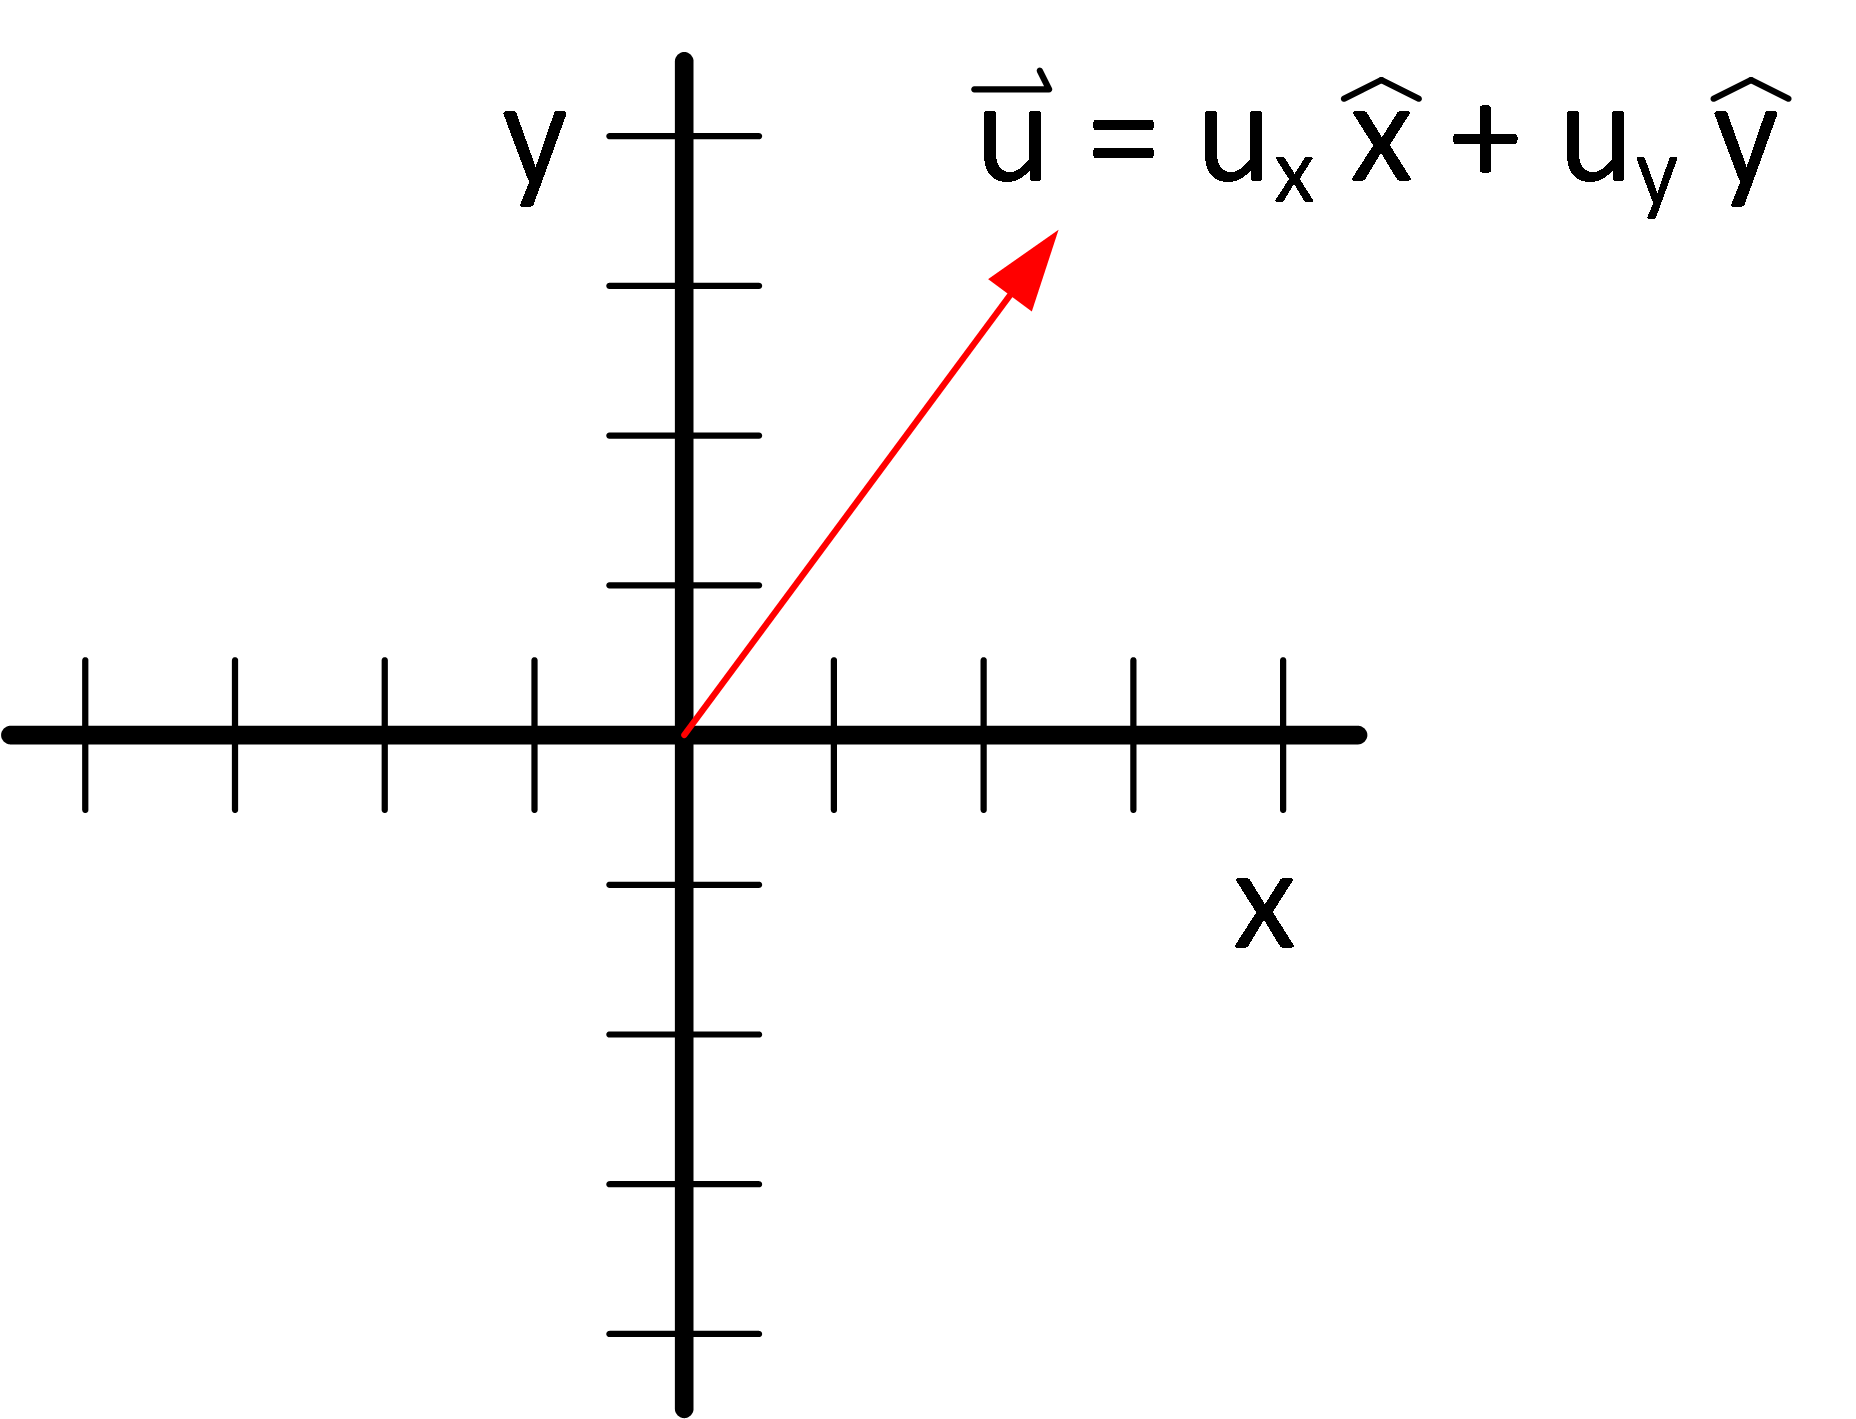
\includegraphics[width=0.4\columnwidth]{2DVectorAsArrowInPlane.png}
	\caption{A 2-dimensional vector represented as an arrow in the plane.}
	\label{fig:2DVectorAsArrowInPlane}
\end{figure}
\begin{figure}[tbh]
	\centering
	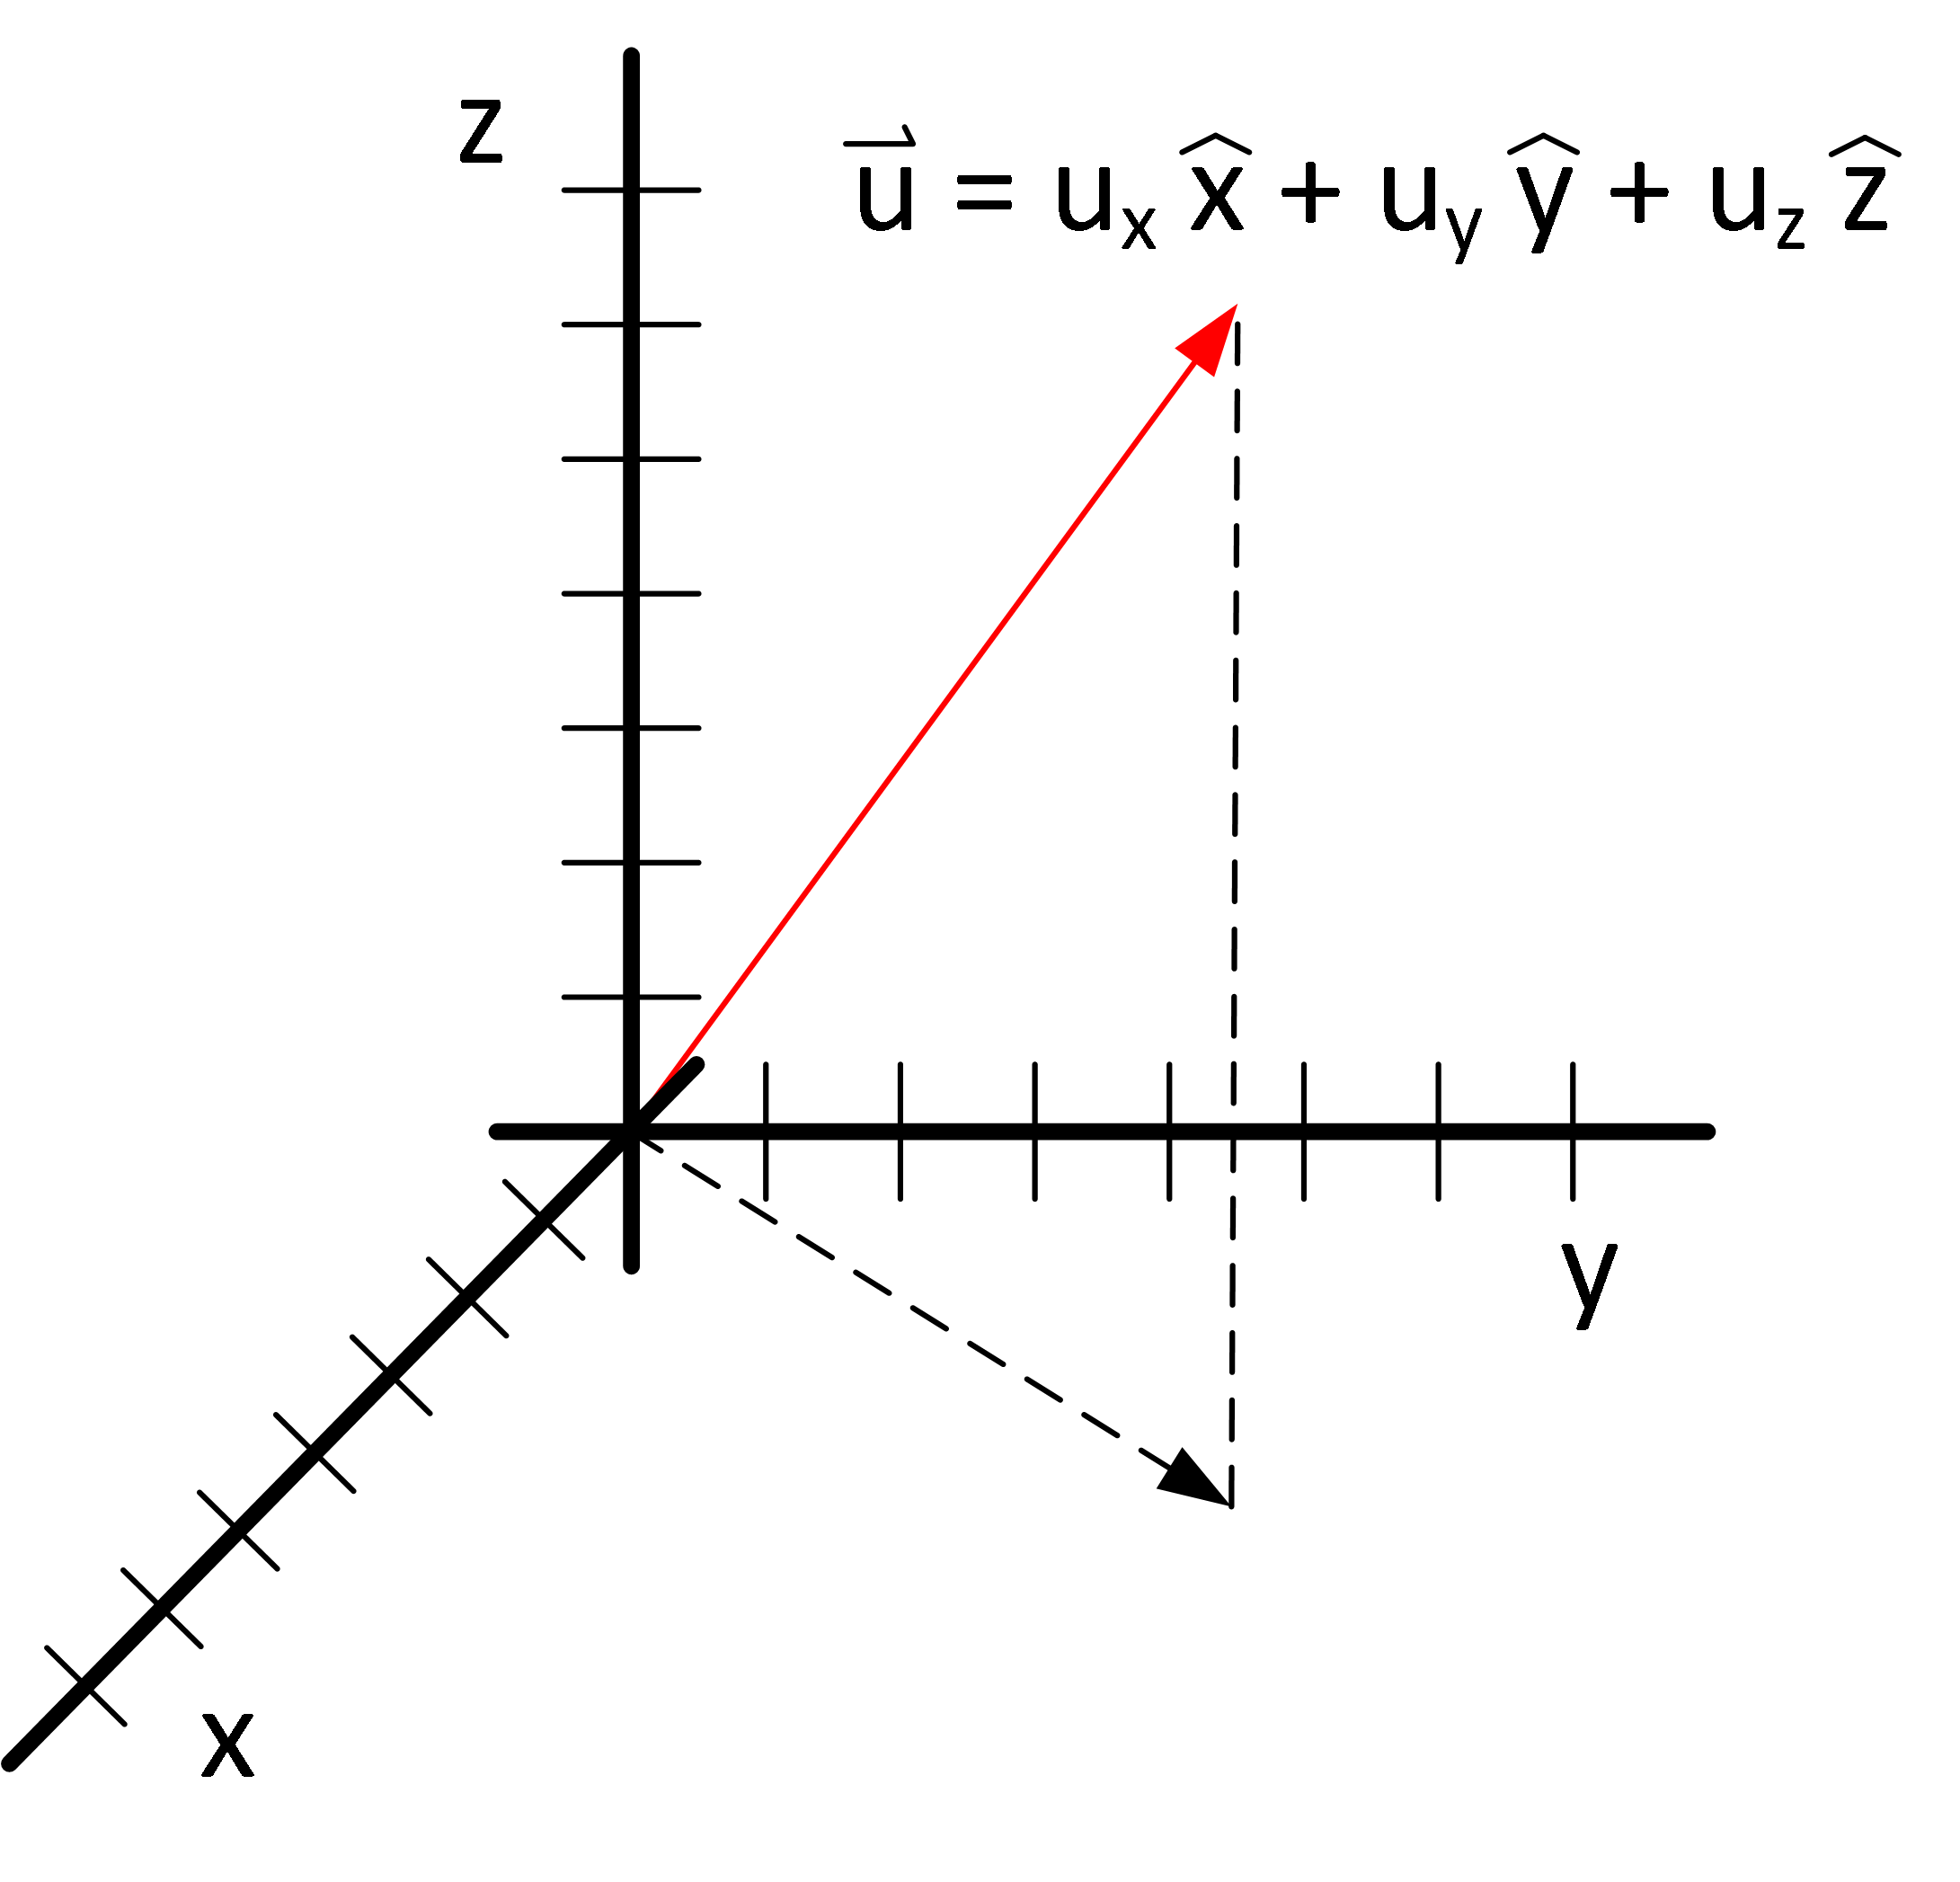
\includegraphics[width=0.6\columnwidth]{3DVectorAsArrowInSpace.png}
	\caption{A 3-dimensional vector represented as an arrow in space.  (The dotted
		arrow is the projection of the 3-vector onto the x-y plane.)}
	\label{fig:3DVectorAsArrowInSpace}
\end{figure}
The length of a vector is commonly called its
norm.  The norm of a vector is computed in the 3-dimensional case as
\begin{equation}
\left\lVert{u}\right\rVert_2 = \sqrt{u_1^2 + u_2^2 + u_3^2} = \sqrt{\sum_{i=1}^3 u_i^2}
\label{eq:normdef}
\end{equation}
More exactly, this is the 2-norm or Euclidian norm of a 3-dimensional vector.
The 2-norm is the most frequently
used vector norm in engineering and physics applications.   
Generalizing the definition of norm to vectors of
higher dimension is an obvious extension of \cref{eq:normdef}.

Visualizing a vector as an arrow in space  
serves well in many disciplines, especially 
in engineering and physics where a vector is used to capture concepts like 
position in real space, particle velocity, the force impressed on a charge by an electric 
field, and so on.  It gives us a way to think about, for example, the 
direction of a force as well as its magnitude.  However, it can also be applied
to more abstract spaces, like a set of measured points $[\xi_1, \xi_2, \xi_3, ... \xi_N] $ taken from an experiment.
That is, a set of $N$ measured points can be thought of as an arrow in some 
$N$-dimensional space, where each measurement $\xi_i$ corresponds to the
amount of that arrow which points in direction $i$.


\section{The matrix as linear transform}
\label{sec:linear_transform}
Visualizing a vector is easy -- the "arrow in space" image is clear
and intuitive.  But how to visualize a matrix?  Is there some geometric
picture which we can carry in our heads which captures important properties
of a matrix?  The answer is "yes" -- that's the subject of this article.
The starting point to visualizing a matrix is
to consider the action of matrix-vector multiplication.  For most of
this article we will work
in 2 dimensions (2x2 matrix), and consider only square matrices.  
That's so we can draw the geometric actions on a two-dimensional page.
In a few examples we will look
at a 3x3 matrix in 3-dimensional space. 
We will also usually use the name $A$ for our matrix, and $u$ and
$v$ as the names of vectors.
Importantly, we will
assume we are looking at a "nice" matrix in a mathematical sense.
That is, we will assume the matrix is
non-singular, has full rank, and so on.  However, the visualizations presented here
also help understanding singular matrices, so later in this article
we will look at some "bad" matrices.  
Finally, extending the geometric concepts
presented here to four and higher dimensions is straightforward -- even if
visualizing an object in four dimensions is difficult for
ordinary human beings!
 

Consider multiplying a 2 element vector $u$ by an arbitrary 2x2 matrix $A$,
$$
v = A u
$$
The result is another 2 element vector $v$.  Consider this operation as
an input-output relationship: the input is the vector $u$ and output is
the vector $v$.  Plot the input vector in the 2D plane in red and the
output vector in the same plane in blue.  The result is shown in
\cref{fig:MatrixVectorMultiplication}.  Multiplication by $A$ has taken the input vector $u$ and
transformed it into the output vector $v$.  
\begin{figure}[thb]
	\centering
	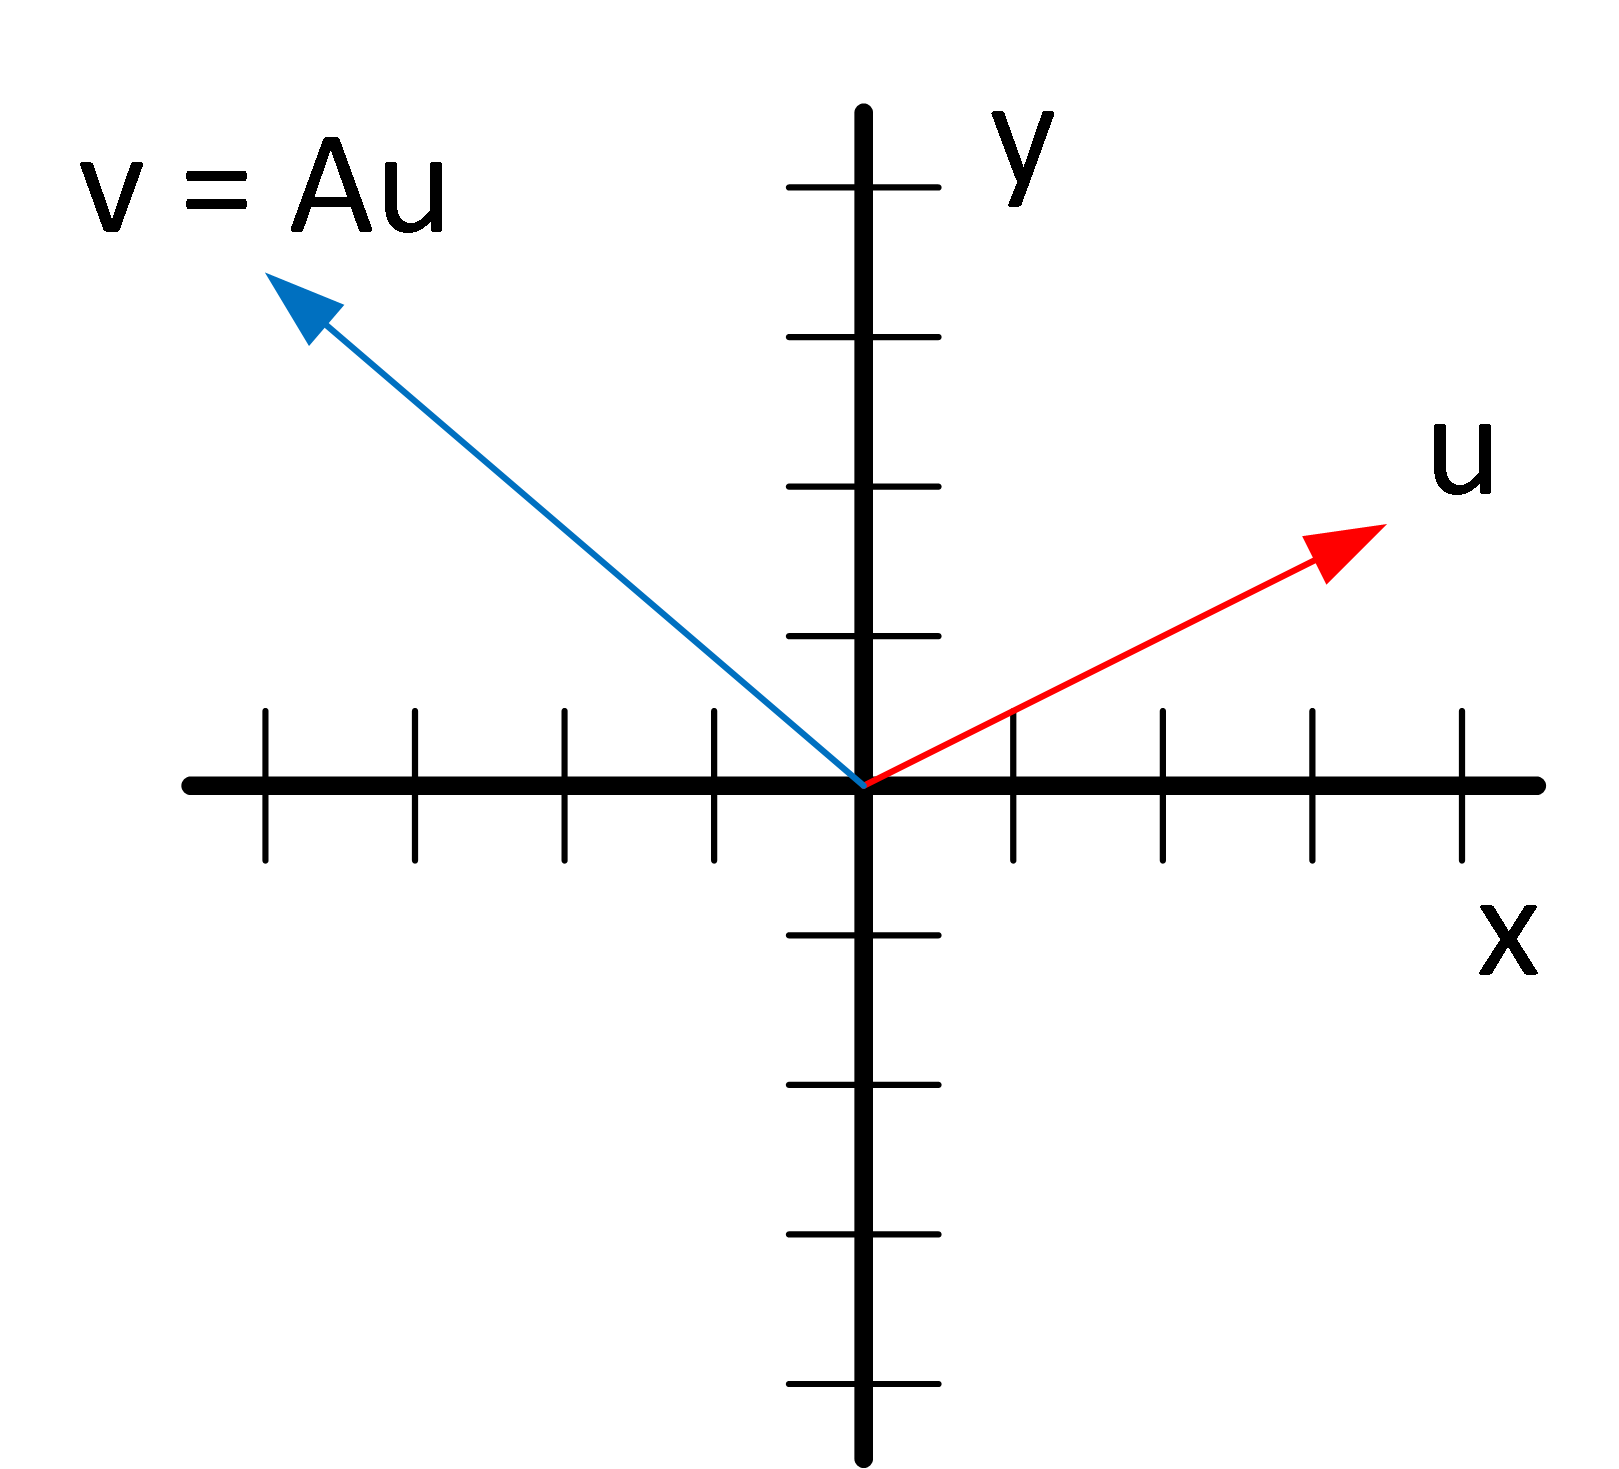
\includegraphics[width=0.4\columnwidth]{MatrixVectorMultiplication.png}
	\caption{Matrix vector multiplication.  The input to this visualization
		is the vector $u$ (red) and the output is the transformed vector $v$ (blue).}
	\label{fig:MatrixVectorMultiplication}
\end{figure}
This is the first way to think about a matrix:  matrix-vector
multiplication is an operation 
which takes a vector and transforms it into a different vector.

\subsection{Abstract linear transform}
An abstract way to think about this is to replace our 2-dimensional
matrix-vector multiplication by the abstract operator $T: \R^2 \to \R^2$ which
takes an input 2-vector $u$ and returns an output 2-vector $v$,
$$
v = T(u)
$$
It can be shown that the operator $T$ is equivalent to matrix-vector multiplication 
as long as the following holds true:
\begin{itemize}
	\item $T(a u) = a T(u)$, where $a$ is a scalar
	\item $T(u+v) = T(u)+T(v)$, where $u$ and $v$ are vectors of the same dimension.
\end{itemize}
These rules are the definition of a linear transform.  Accordingly, matrix-vector
multiplication $v = A u$ may be viewed as implementing a linear transform operation which
takes $u$ to $v$.   
Traditional linear algebra textbooks make a big deal out of this, but for our purposes the important
concept is that we can treat matrix-vector multiplication as implementing
an operation which behaves like a function, $v = T(u)$.  Thought of this way, the
objects of our study are the properties of matrix $A$ itself, 
specifically when $A$ is used as a linear transform $T()$
taking input 2-vectors to output 2-vectors.


\subsection{Transforming a unit square}
\begin{figure}[thb]
	\centering
	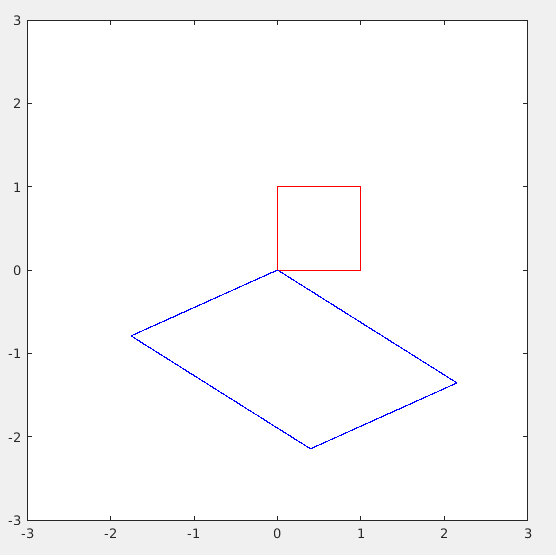
\includegraphics[width=0.7\columnwidth]{MatrixActionOnUnitSquare.png}
	\caption{The action of matrix-vector multiplication on a unit square.  
		The original unit square is red, the transformed square is blue.}
	\label{fig:MatrixActionOnUnitSquare}
\end{figure}
The linear transform picture
\cref{fig:MatrixVectorMultiplication} is frequently featured in 
linear algebra textbooks, so we
won't dwell on it here.  But a useful extension of this
picture involves considering what happens when you draw a square in
the x-y plane, and operate on all its points with the matrix
$A$.  This is shown in \cref{fig:MatrixActionOnUnitSquare}, 
where we create a unit square with
one corner lying at the origin.  We call the input points $u$.
Upon multiplication with the matrix $A$
the input points $u$ are mapped to the output points $v$,
which form a parallelogram.  One vertex of the output parallelogram lies at
the origin -- multiplying the zero
point by $A$ returns zero, so this point doesn't move.  However, all
other points in the input square are mapped to some new point on the
output shape.  What's noteworthy is that the set of output points $v$ always
form a parallelogram (as opposed to forming some other shape).
\FloatBarrier

Matlab code to perform this operation is presented in \cref{mat:ActionUnitSquare}. If
you run this code repeatedly it will generate a new random matrix with
each run, and you will get a different output parallelogram each time.
This is shown in \cref{fig:4Parallelograms}.
\begin{figure}[thb]
	\centering
	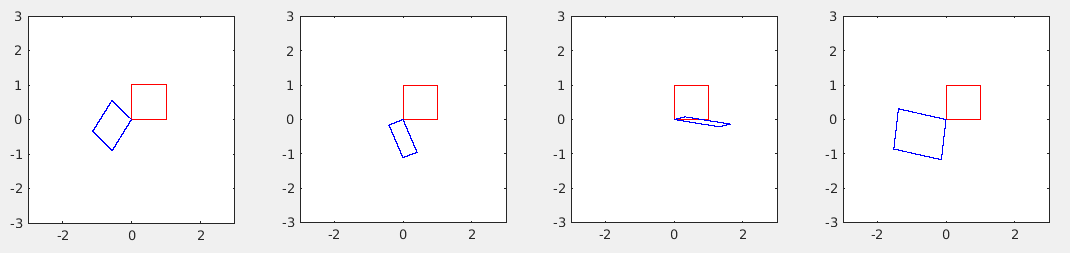
\includegraphics[width=1.0\columnwidth]{4Parallelograms.png}
	\caption{Four different parallelograms generated from four different random matrices.}
	\label{fig:4Parallelograms}
\end{figure}
Examining the results produced by several different matrices shows that
the resulting square is both stretched and rotated by the action of $A$.  This is
an important observation which we will return to in subsequent sections.


Now let's ask an interesting question: what is the area of the
parallelogram generated by $v = A u$?  It turns out the area $D$ is given by
the determinant, $D = \det(A)$.  In our specific 2-dimensional case, if matrix $A$ is 
$$
A = 
\begin{pmatrix}
\alpha & \delta \\
\beta & \gamma
\end{pmatrix}
$$
then we have 
\begin{equation}
D = \det(A) = \alpha \gamma - \beta \delta
\label{eq:detareaformula}
\end{equation}
A "proof without words" of \cref{eq:detareaformula} is shown in \cref{fig:ParallelogramAreaDetFormula}.  
\begin{figure}[thb]
	\centering
	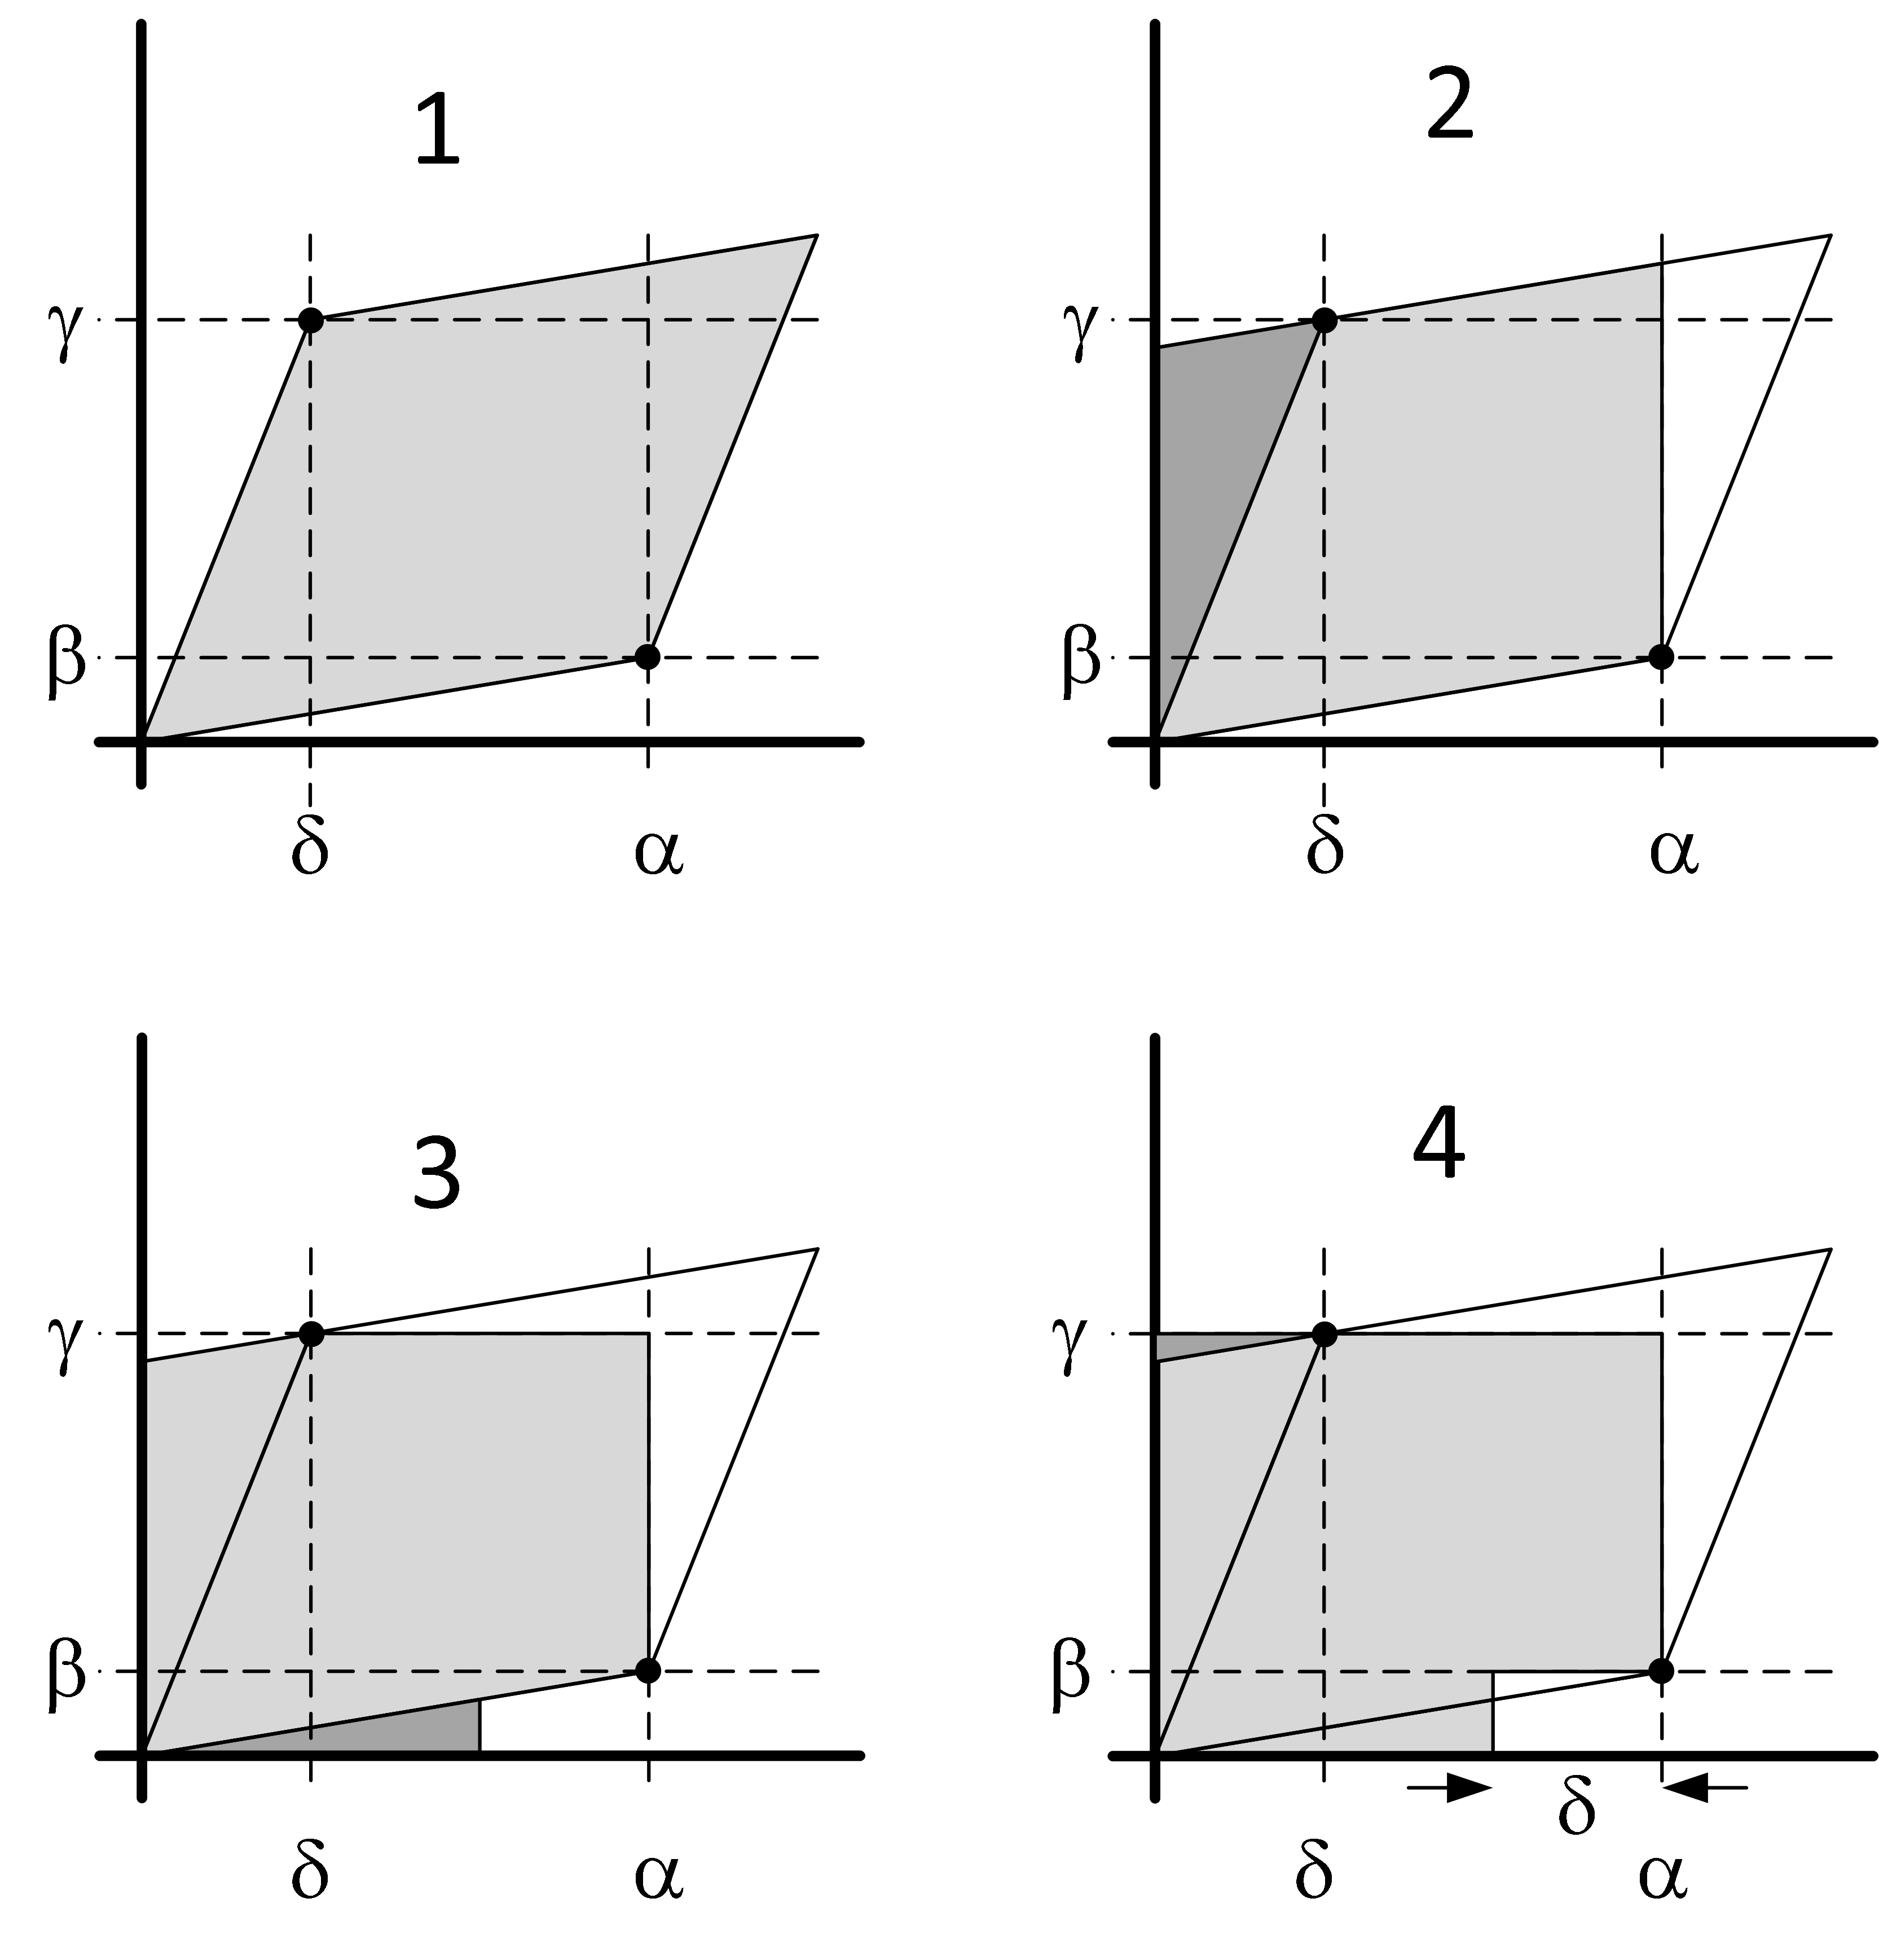
\includegraphics[width=0.7\columnwidth]{ParallelogramAreaDetFormula.png}
	\caption{Proof that the area of the parallelogram created by $v = A u$ is 
		$\det(A) =  \alpha \gamma - \beta \delta$.
	The proof involves performing rigid motions of parts of the parallelogram so the object
	is rearranged into a form where Area = $\alpha \gamma - \beta \delta$ may be deduced by inspection.}
	\label{fig:ParallelogramAreaDetFormula}
\end{figure}
There are a couple of interesting observations to make about \cref{eq:detareaformula}:
\begin{itemize}
	\item If $A$ is singular, then $\det(A) = 0$.  In this case, the parallelogram
	reduces to a line segment with zero area (or possibly even just a point at the origin
	if $A$ is the zero matrix).  Therefore, even with this simple visualization, the concept
	of a singular matrix has a geometric interpretation as a degenerate form of the parallelogram.
	
	\item For some matrices, $\det(A)$ is negative which implies the
	parallelogram area can be negative.  A negative area can seem unintuitive at
	first, but if you think of the order in which the two sides
	are visited you see that one may visit them in two different
	orders:  first right then left, or first left then right.  This
	is similar to computing the "right hand rule" associated with
	the vector cross product.  That is, the area reported by 
	\cref{eq:detareaformula} is a "signed area" which can take on
	either sign depending upon the details of how 
	matrix $A$ is constructed.
\end{itemize}


%%%%%%%%%%%%%%%%%%%%%%%%%%%%%%%%%%%%%%%%%%%%%%%%%%%%%%%%%%%%%5
% Application:  rotation and stretching matrices.
\subsection{Application:  Rotation and stretching matrices}
The transformation shown in \cref{fig:MatrixActionOnUnitSquare} evidences two important
operations performed by the transformation:  rotation and stretching.
That is, the transformation $A u$ has taken the input square, and
stretched it and rotated it to create the output square $v$.
Rotation is a "rigid motion" of an object -- one which moves
the object but doesn't change its shape.  Stretching changes the
object's shape.  (A third effect of matrix multiplication is "inversion", 
which in two dimensions is achieved by flipping the object over.  We'll
ignore inversion for now.)

In two dimensions, the rotation transformation may be captured using
a so-called rotation matrix, frequently written as
\begin{equation}
R(\theta) =
\begin{pmatrix}
\cos \theta & \sin \theta \\
-\sin \theta & \cos \theta
\end{pmatrix}
\end{equation}
Multiplying a vector by this rotation matrix 
rotates it about the origin by the angle $\theta$.  An
example rotation of the square is shown in \cref{fig:RotateASquare}.
\begin{figure}[tbh]
	\centering
	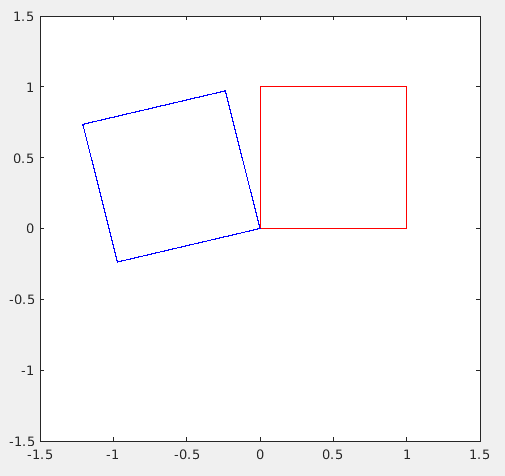
\includegraphics[width=0.7\columnwidth]{RotateASquare.png}
	\caption{Multiplication of the input red square by the rotation matrix $R(\theta)$ takes
		each point and rotates it by angle $\theta$ to
		create the output blue square.}
	\label{fig:RotateASquare}
\end{figure}
There are many noteworthy features of rotation matrices.  Here are three:
% Third:  Q' = Q
\begin{enumerate}
	\item Since rotation is a "rigid motion", it preserves the areas of objects
	being rotated.  This is evident upon inspection of the
	input and output squares shown in \cref{fig:RotateASquare} -- the
	areas of the two squares are the same.
	This implies that the determinant of the rotation matrix
	must be one, which is easily verified:
	$$
	\det(R) = 
	\det \begin{pmatrix}
	\cos \theta & \sin \theta \\
	-\sin \theta & \cos \theta
	\end{pmatrix} =
	\cos^2 \theta - (-\sin^2 \theta) = 1
	$$
	Since the determinant is one, the rotation matrix will preserve
	the area of any object it operates on.  This is a satisfying property
	since intuitively we expect rotation to preserve area.
	
	\item Cascading two rotations by $\theta_1$ (first) and $\theta_2$ (second)
	is equivalent to multiplying the two
	corresponding rotation matrices together.  This can be shown by
	evaluating the matrix multiplication and using trig identities to
	simplify the result.
	\begin{align}
	R(\theta_2) R(\theta_1) =&
\begin{pmatrix}
\cos \theta_2 & \sin \theta_2 \\
-\sin \theta_2 & \cos \theta_2
\end{pmatrix}
\begin{pmatrix}
\cos \theta_1 & \sin \theta_1 \\
-\sin \theta_1 & \cos \theta_1
\end{pmatrix} \nonumber\\
=& \begin{pmatrix}
\cos \theta_2 \cos \theta_1 - \sin \theta_2 \sin \theta_1 & \cos \theta_2 \sin \theta_1  + \sin \theta_2 \cos \theta_1   \\
-\sin \theta_2 \cos \theta_1 - \cos \theta_2 \sin \theta_1 & -\sin \theta_2 \sin \theta_1 + \cos \theta_2 \cos \theta_1 
\end{pmatrix} \nonumber\\
=& \begin{pmatrix}
\cos (\theta_2 + \theta_1) & \sin (\theta_2 + \theta_1) \\
-\sin (\theta_2 + \theta_1) & \cos (\theta_2 + \theta_1)
\end{pmatrix} \nonumber
	\end{align}
	
	\item
	The rotation matrix is a subset of the general set of "orthogonal matrices" \cite{higham2020_OrthoMatrix}.  These
	are matrices made by concatenating orthogonal column vectors like this:
	$$
	\begin{pmatrix}
	\vdots & \vdots & \vdots \\
	q_1 & q_2 & q_3 \\
	\vdots & \vdots & \vdots
	\end{pmatrix}
	$$
	Orthogonal matrices are usually
	notated using the name $Q$ for the matrix.  It is easy to show that orthogonal matrices
	obey the relationship
	\begin{equation}
	Q^T Q = Q Q^T = I
	\label{eq:orthogonalmatrix}
	\end{equation}
	where $I$ is the identity matrix.  The proof is based on looking at the dot products
	of the constituent column vectors -- try doing it yourself!  
	Another way of expressing \cref{eq:orthogonalmatrix} is to recognize that the
	transpose of an orthogonal matrix is its inverse,
	$$
	Q^T = Q^{-1}
	$$
	These facts become useful when studying matrix decompositions such as the SVD, the EVD,
	and the QR decomposition, which yield an orthogonal matrix as one of the factors.
\end{enumerate}

Another possible action produced by the transformation $A u$ is stretching.
For simplicity we specialize to the case of a diagonal matrix,
\begin{equation}
D = 
\begin{pmatrix}
d_1 & 0 \\
0  & d_2
\end{pmatrix}
\end{equation}
The action of $D$ is to stretch the $x$ axis by factor $d_1$ and the
$y$ axis by factor $d_2$.  This is shown in \cref{fig:StretchASquare}
below, which depicts the action of the matrix 
$D = \bigl( \begin{smallmatrix} 1.5 & 0 \\ 0 & 0.8\end{smallmatrix}\bigr)$
on the unit square.  By inspection it is evident the square grows in the $x$ direction
by $1.5$ and shrinks in the $y$ direction by $0.8$; the output
is a rectangle.

We will examine the case of stretching in arbitrary directions in 
section \cref{rotstretchrot} below, which describes the singular value decomposition.

\section{Transforming a unit circle}
\label{sec:unit_ball}
In the last section we examined the action of a 2x2 matrix on the unit
square.  Rather than visualizing the matrix directly, we looked at its
effect on a square in the x-y plane.  In this section we look at the
effect of a 2x2 matrix on a unit circle (unit ball) in the x-y plane.

Consider how to plot the points on a unit circle.  
The most common definition of the unit circle is 
that it is the locus of all points in the x-y
plane satisfying
\begin{equation}
x^2 + y^2 = 1
\label{eq:unit_ball}
\end{equation}
One can imagine every point on the circle is represented as the tip
of a unit length vector.  If you take the collection of unit vectors
based at the origin and pointing in all different directions, 
the set of all vector tips 
define a circle.  Therefore, a different way to 
create a plot of the unit circle is use a parametric
representation.  Consider all vectors of form
\begin{equation}
u = 
\begin{pmatrix}
x \\
y 
\end{pmatrix}
=
\begin{pmatrix}
\cos(\theta) \\
\sin(\theta) 
\end{pmatrix}
\label{eq:parametriccircle}
\end{equation}
where $\theta \in [0, 2\pi]$.  

\begin{figure}[thb]
	\centering
	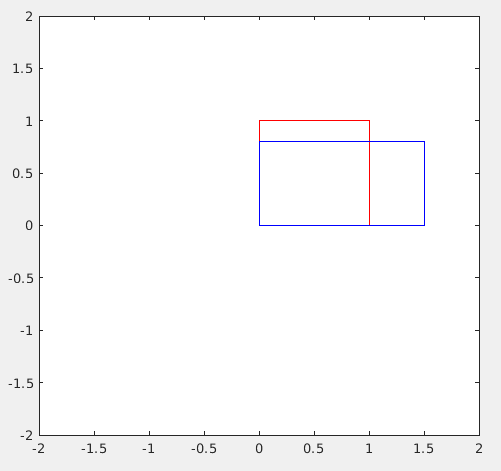
\includegraphics[width=0.7\columnwidth]{StretchASquare.png}
	\caption{Multiplication by diagonal matrix 
	$D = \bigl( \begin{smallmatrix} 1.5 & 0 \\ 0 & 0.8\end{smallmatrix}\bigr)$
	stretches the input square (red) in the $x$ and $y$ directions. The
	result is the output rectangle (blue).}
	\label{fig:StretchASquare}
\end{figure}
\FloatBarrier



Each point $u = (x(\theta), y(\theta))^T$ 
satisfies \cref{eq:unit_ball}, so each of these points lies on the
unit circle.  Therefore, this representation provides a
simple algorithm to create a unit circle in the plane:  just sweep 
$\theta$ from $0$ to $2\pi$ and plot the points $(x(\theta), y(\theta))^T$.

Now we will use the set of unit vectors created by \eqref{eq:parametriccircle}
to create a visualization for a matrix.
This visualization considers how the circle of unit vectors is itself
transformed by matrix-vector multiplication.  The idea is to take
every unit vector $u$ and multiply by the matrix $A$, giving a
new point $v$.  Then plot the set of all points $v$ generated by $v = A u$.  
A Matlab program which implements this idea is given in \cref{Mat:ActionUnitBall}.  The circle and its
transformed image are shown in \cref{fig:CircleTransformedToEllipse}.
\begin{figure}[thb]
	\centering
	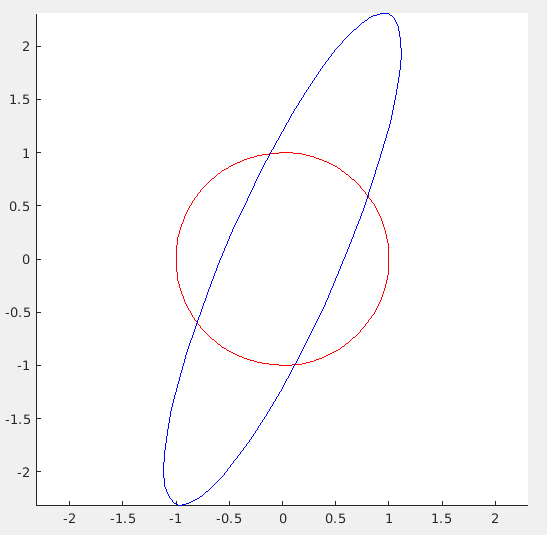
\includegraphics[width=0.7\columnwidth]{CircleTransformedToEllipse.png}
	\caption{Multiplication by matrix $A$ sends every point on the unit circle to a point on an ellipse.}
	\label{fig:CircleTransformedToEllipse}
\end{figure}
The important thing to note in \cref{fig:CircleTransformedToEllipse} is that the circle has been
transformed into an ellipse.  The shape, size, and rotation of the ellipse are given
by the properties of the matrix $A$.  Different matrices will create different
ellipses having different shapes, sizes, and rotations.  This is illustrated
by running the program in \cref{Mat:ActionUnitBall} several times for different, randomly generated
$A$ matrices.  The results obtained by operating on a circle using four different random matrices 
are shown in \cref{fig:4Ellipses}
\begin{figure}[thb]
	\centering
	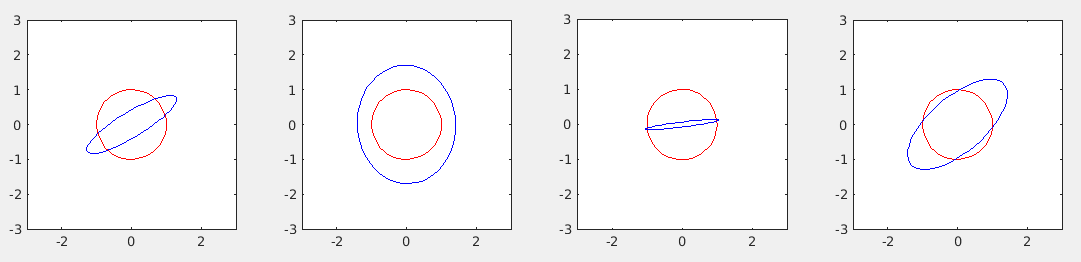
\includegraphics[width=1.0\columnwidth]{4Ellipses.png}
	\caption{Repeated runs of the unit circle program produce different random matrices $A$ which 
		product different output ellipses.  The original unit circle is red, the output ellipses are blue.}
	\label{fig:4Ellipses}
\end{figure}

It may appear this matrix visualization involving
transforming unit circles into ellipses is similar to the
visualization involving the unit square and is therefore redundant.  
However, that is not true -- several very deep properties of a matrix are
better understood by investigating the ellipse
visualization.  Investigating these properties is the task of the following subsections.

\subsection{Matrix norm}
In general, the norm of any mathematical object 
is an operation which takes the object and maps it
to a positive real scalar.  The size of the scalar tries to measure something
related to the magnitude of the object -- the norm gives a measure how
"big" the object is in some sense.  
For example, the familiar vector norm measures
the length of the "arrow in space".  The general goal of defining a norm on some
object is to capture the idea of "bigness" in a way which is useful
in calculation.

When defining the norm of a new mathematical object, one must take
care to satisfy a set of rules about the behavior of a norm.
The purpose of the rules is to ensure
that the so-defined norm not only measures the
"bigness" of the object under consideration, but is also sane.  
Also, the rules make it possible to compare
the "bigness" of two different objects using their norms in a
meaningful way.

Here are the rules for creating a norm.  They are abstract rules, meaning
they hold when computing the norm of any object, whether a vector, a matrix, or
some other mathematical construction.
If $M$ and $N$ are two of the objects under consideration, their 
norms must satisfy
\begin{itemize}
	\item $\left\lVert{M}\right\rVert \geq 0$
	
	\item $\left\lVert{a M}\right\rVert = \left\lvert{a}\right\rvert\left\lVert{M}\right\rVert$
	
	\item $\left\lVert{M+N}\right\rVert \leq \left\lVert{M}\right\rVert + \left\lVert{N}\right\rVert$
	
	\item if $M$ is a zero object, then $\left\lVert{M}\right\rVert = 0$.
\end{itemize}
We note that these rules leave a lot of flexibility for defining a
norm.  This flexibility manifests itself when considering computing
the norm of a vector -- there are many different ways to compute a
vector norm, including:
\begin{itemize}
	\item $L_1$ norm: $\left\lVert{x}\right\rVert = \sum_i \lvert x_i\rvert$
	
	\item $L_2$ (Euclidian) norm: $\left\lVert{x}\right\rVert = \sqrt{\sum_i x_i^2}$
	
	\item $L_\infty$ norm: $\left\lVert{x}\right\rVert = \max\limits_{i} \lvert x_i \rvert$
\end{itemize}

Although having multiple ways to compute a norm might seem redundant,
it turns out that different vector norm definitions find application
in different places, depending upon the needs of the application and the properties
of the particular norm. 

What about the norm of a matrix?  Similar to vector norm,
there are several ways to define a
matrix norm \cite{Weisstein_MatrixNorm}.  One particularly useful definition generates the
so-called "induced norm", which measures how much the matrix $A$ can
stretch a vector.  Since this matrix norm is based on computing vector
norms, one can think of this definition as  "induced" by the
definition of the vector norm, hence the name.


The induced matrix norm is found as follows.  Consider an input vector
$u$ with norm $\left\lVert {u}\right\rVert$.  We use the Euclidian ($L_2$) norm for the vector
norm.  Now consider operating on $u$ with $A$ via matrix-vector
multiplication, $v = A u$.
The output vector $v$ will also have a norm,  $\left\lVert {v}\right\rVert$.  Now ask, what is the
relationship of  $\left\lVert{u}\right\rVert$ to  $\left\lVert{v}\right\rVert$?  
Performing this computation is easy.
The action of $A$ on $u$ is to stretch and rotate it, giving the output
vector $v$.
This is where you can see the idea of the
"bigness" of $A$ coming to play -- if $A$ doesn't stretch $u$ by very much,
then we can think of $A$ as not particularly big.  But if $A$ stretches $u$
by a lot, then we can think of $A$ as "big".  
Therefore, the definition of matrix norm, $\left\lVert{A}\right\rVert$,
should reflect that notion.


To capture the notion of "bigness" we ask, what is the maximum
amount of stretching caused by $A$?  To find this, consider rotating $u$
around the origin while leaving its magnitude fixed.  Then look at the
length of the transformed vector $v = A u$.  In the general case, this
vector will have a maximum length for some input vector $u$.  The norm
of $A$ will then be the ratio of the output to the input vector lengths:
\begin{equation*}
  \label{eq:inducednorm}
\begin{aligned}
\left\lVert {A}\right\rVert 
& = \argmax_u \frac{\left\lVert{v}\right\rVert}{\left\lVert{u}\right\rVert} \\
& = \argmax_u \frac{\left\lVert{A u}\right\rVert}{\left\lVert{u}\right\rVert}
\end{aligned}
\end{equation*}
This is the definition of induced matrix norm ordinarily found in
textbooks.  Although it looks intimidating, it really says something simple.
It says, rotate the input vector $u$ around the origin and look for the
output vector $v$ of maximum length.  
Then, take the ratio of the two vector lengths to get the matrix norm.
The factor of 
$\left\lVert{u}\right\rVert$ in the
denominator is just a normalization factor -- it says that if $u$ is not
a unit vector, then the output value should be scaled by the length of $u$.
\begin{figure}[H]
	\centering
	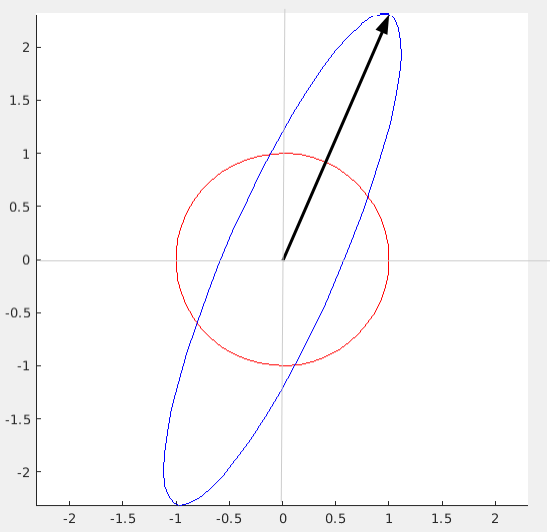
\includegraphics[width=0.6\columnwidth]{InducedMatrixNormWithArrow.png}
	\caption{The induced matrix norm of $A$ is the length of the longest vector
		lying on the surface of the ellipse generated by the matrix-vector
		product $v = A u$, where $u$ is a unit vector.}
	\label{fig:InducedMatrixNormWithArrow}
\end{figure}
\FloatBarrier 

A better way to understand this definition of matrix norm is to appeal
to the ellipse visualization presented earlier in this section.
Using the ellipse visualization, the norm of $A$ is the length
of the ellipse's semi-major axis.  
This is shown in 
\cref{fig:InducedMatrixNormWithArrow}, 
where the arrow identifies the semi-major axis. 
The length of this arrow is exactly 
the norm of $A$.

\subsection{Singular value decomposition and the ellipse visualization}
The singular value decomposition (SVD) of a matrix is an operation
which may be considered as a generalization of the eigenvalue
decomposition (EVD) \cite{higham2020_svd}.   Unlike the EVD, however, a matrix always has an
SVD, regardless of whether it is square or rectangular, singular or
not.  The SVD separates the
matrix $A$ into three different factors (pieces).  The decomposition performed
by the SVD is
$$
A = U \Sigma V^T
$$
where $U$ and $V$ are orthogonal matrices, and $\Sigma$ is a diagonal matrix.
The elements on the diagonal of $\Sigma$ are denoted by $\sigma_i$ and are
called the "singular values" of matrix $A$.  More information about the
SVD is available in many linear algebra textbooks, so I will assume
you already know about the SVD.


The ellipse visualization of matrix $A$ is related to its SVD on several
levels.  The first relationship is simple:  The two singular values of
$A$ are the lengths of the semi-major and semi-minor axes of the
ellipse.  This is shown in \cref{fig:EllipseAxes}, where the semi-major and
semi-minor axes are indicated by arrows.
\begin{figure}[H]
	\centering
	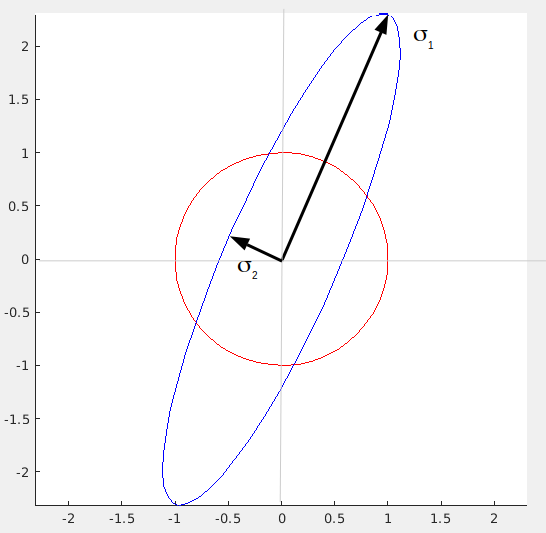
\includegraphics[width=0.8\columnwidth]{EllipseAxes.png}
	\caption{The lengths of the semi-major and semi-minor axes of the ellipse
		are given by the singular values of $A$: $\sigma_1$ and $\sigma_2$.
		The input circle is red, the output ellipse is blue.}
	\label{fig:EllipseAxes}
\end{figure}
\FloatBarrier

This property of the SVD generalizes to $N$ dimensions -- for an $N \times N$ matrix 
consider the ellipsoid created by matrix-vector multiplication with the unit ball (sphere), $v = A u$.
Again, $u$ is the set of unit vectors in N-space.
The length of each semi-axis of the
output ellipse $v$ is given by the corresponding singular value in the SVD
of $A$.   \cref{fig:3DEllipse} shows a 3-dimensional unit ball and the resulting
ellipsoid computed using the visualization library VTK.  The numeric values
of $\sigma_i$ are also shown in the figure.

\begin{figure}[H]
	\centering
	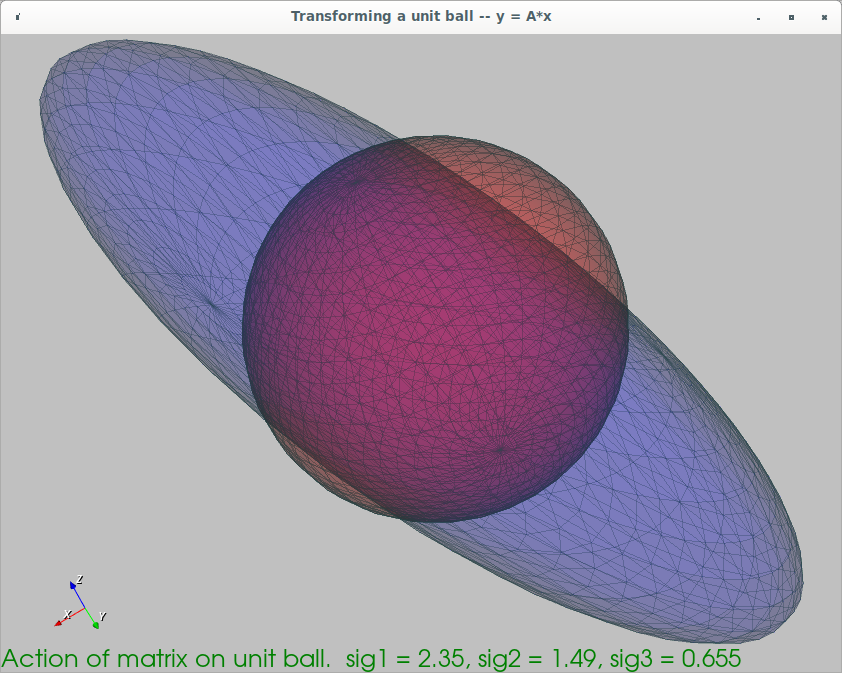
\includegraphics[width=0.8\columnwidth]{3DEllipse.png}
	\caption{
		For the 3-dimensional ellipsoid created by $A u$ the
		lengths of the axes of the ellipse
		are given by the singular values of $A$: $\sigma_1$, $\sigma_2$, and $\sigma_3$.
		The input sphere is red, the output ellipsoid is blue.}
	\label{fig:3DEllipse}
\end{figure}
\FloatBarrier 


\subsection{The full action of SVD -- rotation, stretching, rotation}
\label{rotstretchrot}
The last subsection showed the relationship of the singular values 
of $A$ to the lengths of the axes of the ellipse created by $v = A u$.
There is much more to the relationship.  Consider the action of the decomposed
matrix $A$ on the unit circle,
\begin{equation}
v = A u = U \Sigma V^T u
\end{equation}
Both $U$ and $V$ are orthogonal matrices.  Therefore, the action of $A$ on $u$
can be visualized as a three-step transformation:
\begin{enumerate}
	\item Multiplication by $V^T$.  Since $V$ is orthogonal (as is $V^T$),
	the operation $V^T u$ corresponds to rotating the circle with no stretching.
	\item Multiplication by $\Sigma$.  Since $\Sigma$ is a diagonal matrix, its action
	is to stretch the circle in the directions of the 
	underlying coordinate axes (i.e. the basis spanning the space of $A$).
	The stretching action is what creates the output ellipse from an input circle.
	\item Multiplication by $U$.  Again,  because $U$ is orthogonal, multiplication
	by $U$ corresponds to taking the ellipse and rotating it.
\end{enumerate}
This three-step action is shown in \cref{fig:ActionOfSVDOnCircle} 
\begin{figure}[thb]
	\centering
	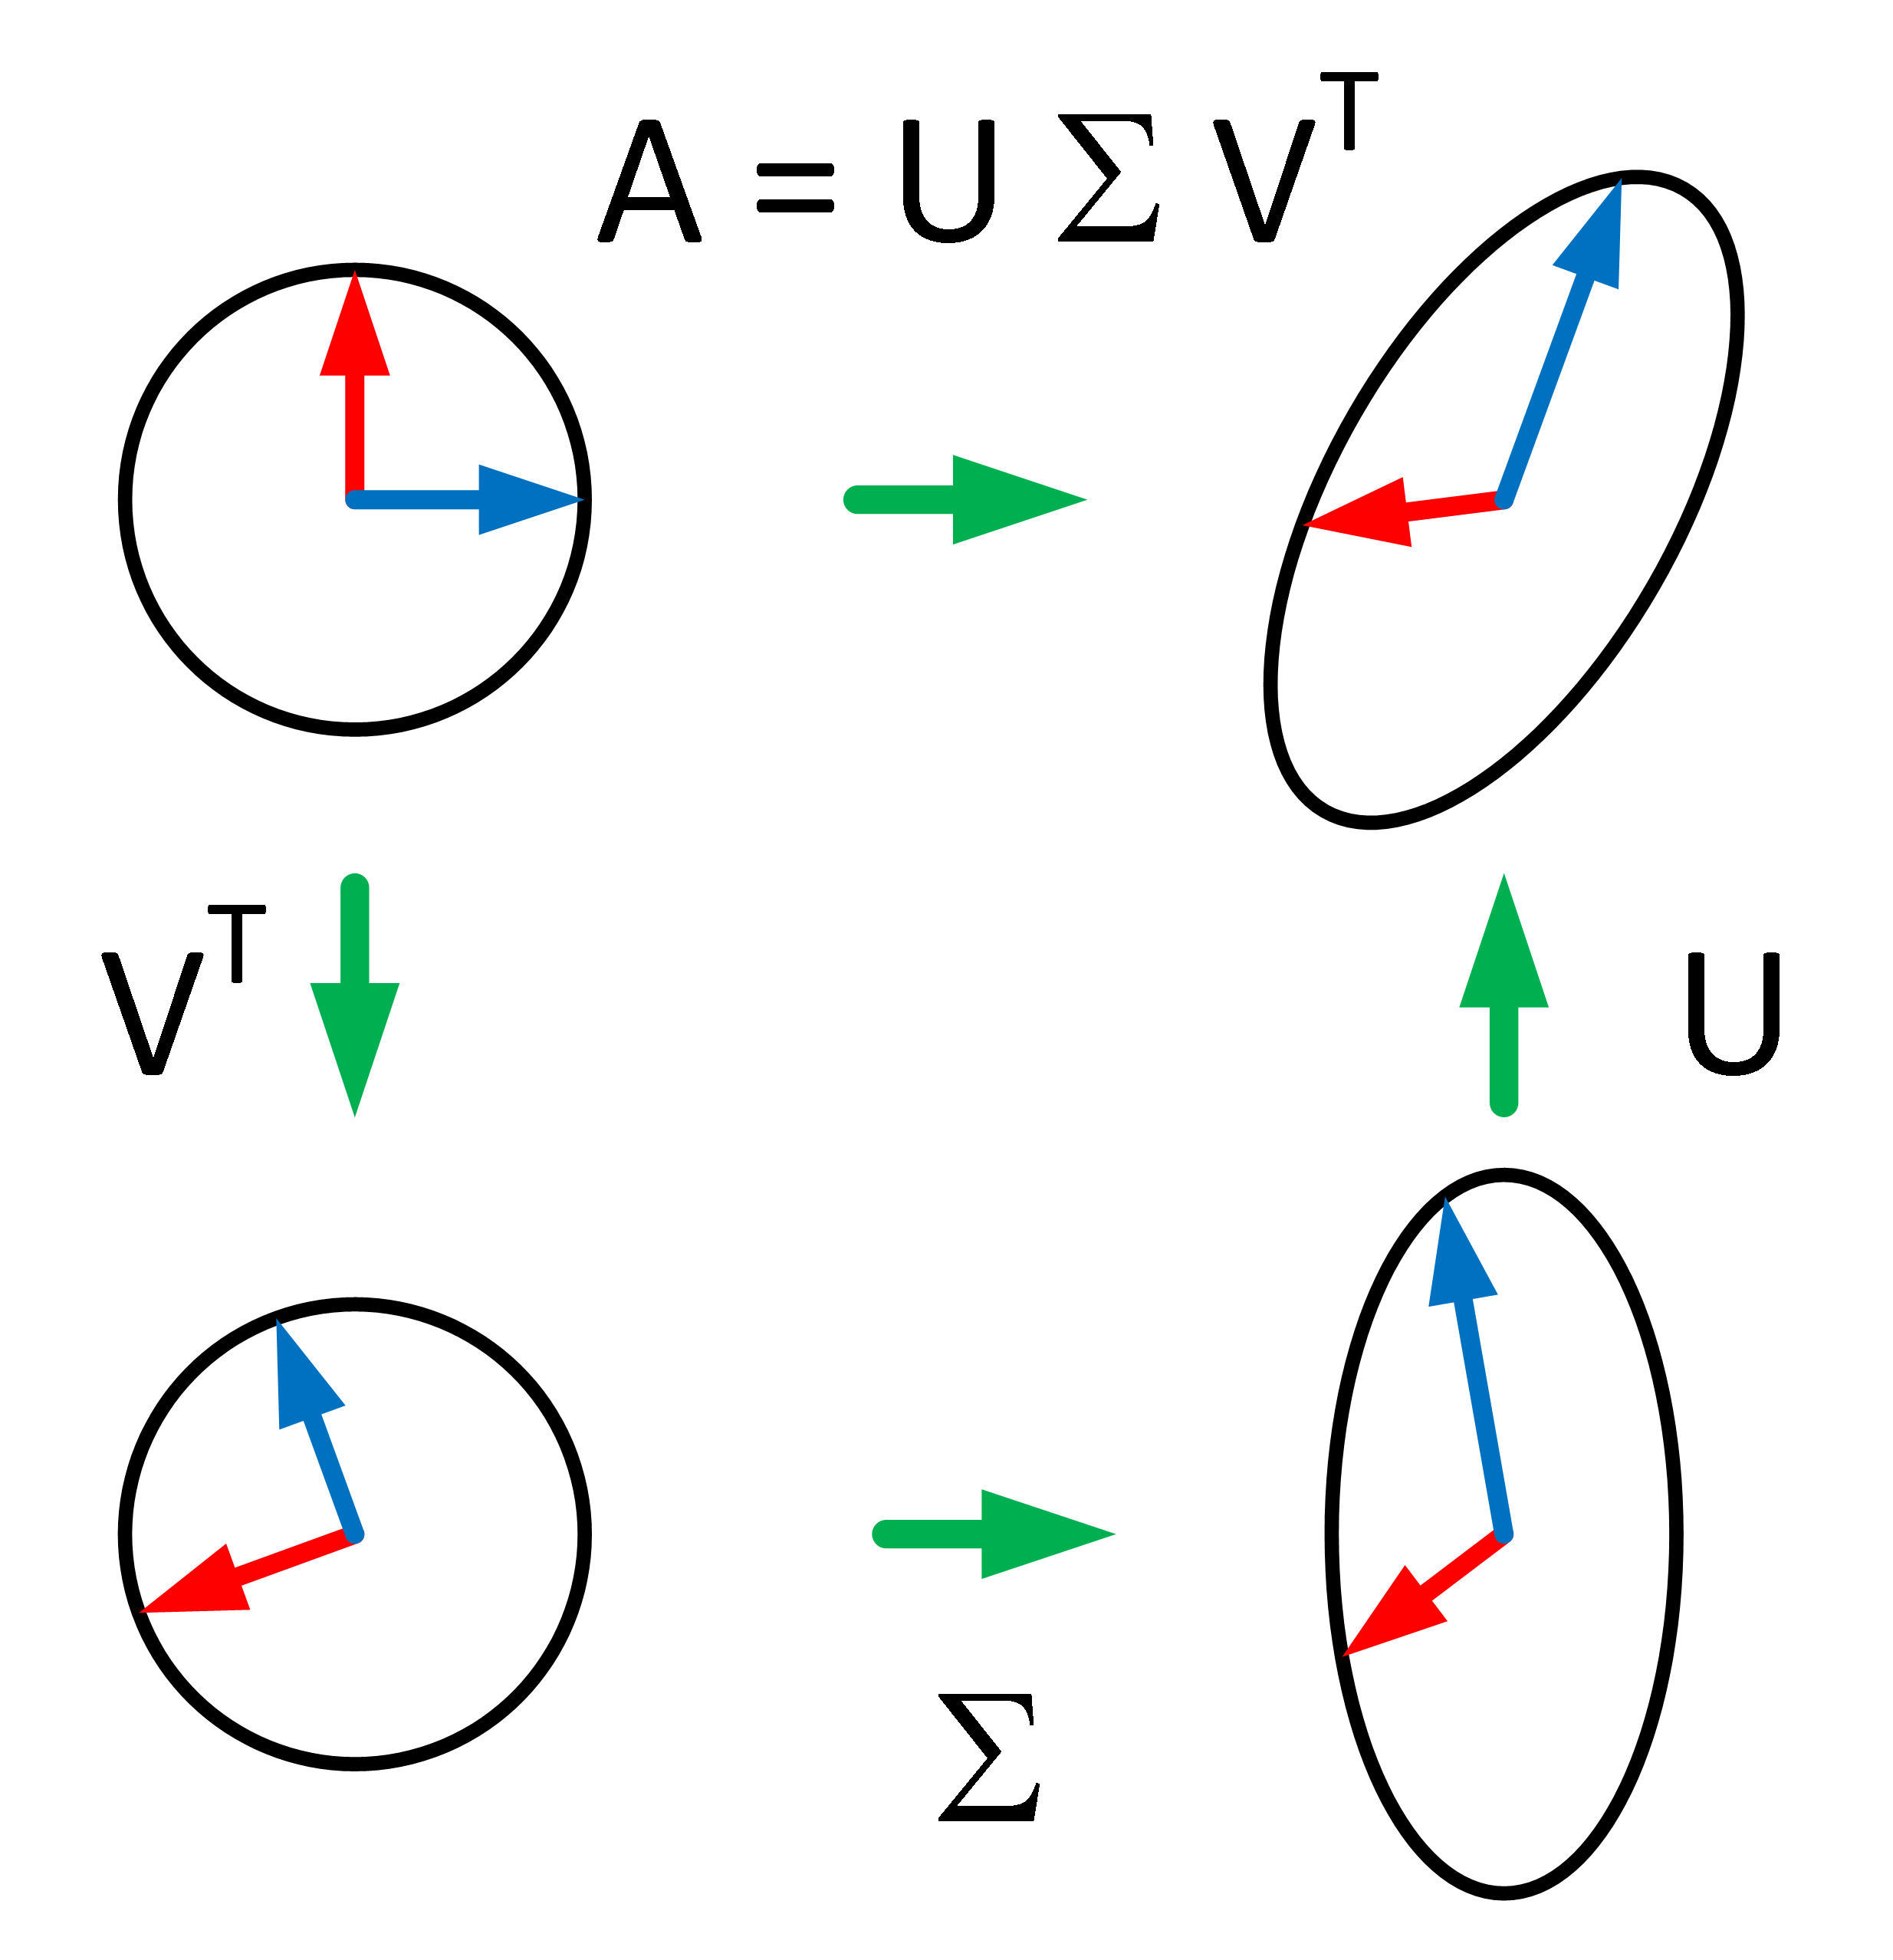
\includegraphics[width=0.4\columnwidth]{ActionOfSVDOnCircle.png}
	\caption{The action of $A$ decomposed into the three steps implemented by the SVD.
	The first action is rotation via the orthonormal matrix $V^T$, then stretching
	via the diagonal matrix $\Sigma$, and finally a second rotation via the orthonormal
	matrix $U$.}
	\label{fig:ActionOfSVDOnCircle}
\end{figure}
The net result of these three transformations is to take a unit circle
and transform it into an ellipse as we have already seen.  Now we see the 
fact that the ellipse's axis lengths are given by the singular values of $A$
is a natural consequence of multiplication by the diagonal matrix 
$\Sigma = \bigl( \begin{smallmatrix}  \sigma_1 & 0 \\ 0 & \sigma_2 \end{smallmatrix}\bigr)$
-- the ellipse
is stretched along axis $i$ by $\sigma_i$.
Additionally, we also see
why the output ellipse is tilted:  the tilt of the ellipse is due to
rotation by $U$ as the final step of the three-step transformation.

One final point is worth mentioning:  In the last subsection we found that
the induced norm of $A$ is the length of the semi-major axis of the ellipse $v$.
Since the ellipse is created by the stretching operations implemented by
$\Sigma$, the longest axis is created by the largest singular value, $\sigma_1$.
Therefore, the induced norm of $A$ is also given by the largest singular value, i.e.
$\left\lVert{A}\right\rVert = \sigma_1$.


\subsection{Condition number}
\label{conditionnumber}
Another important property of a matrix $A$ is its condition number \cite{moler2017}.  The
condition number of a matrix is a scalar which characterizes how close
the matrix is to singular.  One usually writes the Greek letter $\kappa$ 
to stand for the condition number.  The condition number is a measure of how
sensitive the linear system
\begin{equation}
  \label{eq:linearsystem}
Ax = b
\end{equation}
is to small perturbations of $A$ and $b$.  In general, the value 
of $x$ obtained by solving \cref{eq:linearsystem} will be 
inexact due to rounding error and other numerical non-idealities.
You might think that if $A$ is close to singular, the
error incurred in solving \cref{eq:linearsystem} will be larger than
if $A$ is far from singular.  This is indeed the case in  
practice, and condition number $\kappa$ quantifies this effect.

The condition number is traditionally defined via
\begin{equation}
\label{eq:condno}
\kappa = {\left\lVert A^{-1} \right\rVert}  {\left\lVert A \right\rVert}
\end{equation}
although using this expression to actually compute a value for
 $\kappa$ is generally
discouraged.  (The reason is that computing the matrix inverse $A^{-1}$
is an $O(n^3)$ operation, while the condition number is more easily
computed using the SVD, which is typically calculated
iteratively.)  Nonetheless, you can see from \cref{eq:condno}
the general behavior of $\kappa$.  On one hand, the most stable matrix
is the identity matrix,
$$
I = 
\begin{pmatrix}
1 & 0 & 0 & 0 \\
0 & 1 & 0 &  \ddots \\
0 & 0 & \ddots & 0 \\
0 & \ddots & 0 & 1
\end{pmatrix}
$$
and for this matrix it's easy to see that the condition number is $\kappa = 1$.  (You can use the unit circle matrix visualization to see why this is true.)
On the other hand, if $A$ is singular, then ${\left\lVert A^{-1} \right\rVert}
= \infty$, so the condition number is also $\infty$.  Therefore, the condition
number of any matrix will lie somewhere in the domain $1 \leq \kappa \leq \infty$.
The condition number is a reliability measure for the solution $x$ of 
the linear system $A x = b$:
\begin{itemize}
	\item The smaller the condition number (closer to 1), the better behaved is
	the matrix.  That means that solving $A x = b$ will give good results for $x$.
	In this case one says the matrix is "well conditioned".
	\item The larger the condition number (closer to $\infty$), the closer
	is the matrix to singular.  In this case, solving the system $A x = b$ 
	is very sensitive to small changes in $A$ and $b$ (i.e. from round-off) so
	the result $x$ may have large errors.  In this case one says the matrix is
	"badly conditioned".
\end{itemize}
This language extends to
numeric problems themselves -- one can speak of well or 
badly conditioned problems.

Having examined some properties of the condition number it's time to actually
compute it.  It turns out that the condition number of matrix $A$ is intimately related
to its SVD.  In particular, the condition number of $A$ is equal to
the ratio of the largest to the smallest singular values of $A$.  That is,
if
$$
A = U 
\begin{pmatrix}
\sigma_1 & 0 & 0 & 0 \\
0 & \sigma_2 & 0 & \ddots \\
0 & 0 & \ddots & 0 \\
0 & \ddots & 0 & \sigma_N
\end{pmatrix}
V^T
$$
then
$$ 
\kappa = \sigma_1 /  \sigma_N 
$$
This can be seen by considering \cref{eq:condno}.  The norm of $A$ is 
the largest singular value $\sigma_1$.  Meanwhile, taking the
SVD of $A^{-1}$ yeilds
\begin{equation*}
\begin{aligned}
A^{-1} & = (U S V^T)^{-1} 
& = (V^T)^{-1} S^{-1} U^{-1}
& = V S^{-1} U^T
\end{aligned}
\end{equation*}
and since $S$ is diagonal we have
\begin{equation}
S^{-1} = 
\begin{pmatrix}
1/\sigma_1 & 0 & 0 & 0 \\
0 & 1/\sigma_2 & 0 &  \ddots \\
0 & 0 & \ddots & 0 \\
0 & \ddots & 0 & 1/\sigma_N
\end{pmatrix}
\end{equation}
Accordingly, the norm of $A^{-1}$ is its largest singular value, 
which is $1/\sigma_N$.  Therefore, from the definition \cref{eq:condno} we have
 $\kappa = \sigma_1 /  \sigma_N$.

What does this mean for our ellipse visualization?  It means that the condition
number of $A$ may be read directly from the shape of the ellipse.
If the ellipse is close to circular in shape, then the matrix is well
conditioned.  But if the ellipse is elongated and skinny, then the matrix
is badly conditioned.  This is illustrated in \cref{fig:EllipsesWithCondNo}
which shows a series of ellipses corresponding to randomly generated
matrices $A$.  Note that the round ellipses have smaller condition numbers
than the skinny ones.

\begin{figure}[thb]
	\centering
	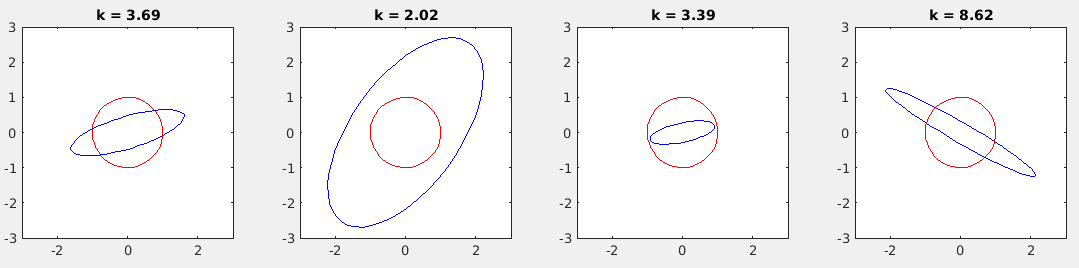
\includegraphics[width=1.0\columnwidth]{EllipsesWithCondNo.png}
	\caption{Ellipses created by different, random matrices $A$.  Ellipses
		which are closer to circular have smaller condition numbers $\kappa$
		while ellipses which are skinnier have higher condition numbers.}
	\label{fig:EllipsesWithCondNo}
\end{figure}

This picture extends to a general N-dimensional
ellipsoid -- if the ellipsoid is close to spherical, the matrix is
well conditioned.  But if the ellipsoid is squeezed or close to flat in one or more
dimensions, then the corresponding matrix is close to singular.
In the limit that the matrix is singular, one or more of the singular 
values are exactly zero, and the corresponding ellipsoid is completely flat in
those directions.  If the ellipsoid looks like a pancake then the matrix
is singular!


%%%%%%%%%%%%%%%%%%%%%%%%%%%%%%%%%%%%%%%%%%%%%%%%%%%%%%%%%%%%%%%%%%%%%%%%%%%
% Application: cond. no and linear solve.
\subsection{Application: Sensitivity of linear solve}
Let's look further into what the condition number $\kappa$ says about
the solution to $A x = b$.
Consider solving this system on a computer
using floating point doubles \cite{Moler2014_FloatingPoint}.  The mantissa of a double is 53 bits
long, which corresponds to roughly 16 decimal digits.
If no errors are introduced using doubles to
represent the known objects $A$ and $b$, then the solution $x$ should be
valid to around 16 decimal digits.  However, errors always creep in to a computer
computation performed with finite-length words.

The linear solve operation takes as input the matrix $A$ and the RHS (right
hand side) vector
$b$, and outputs the vector $x$ which satisfies $A x = b$.  Now imagine 
we could calculate the solution $x$ exactly -- without any rounding error.
What is the difference between this "mathematically true" solution $x$ and the 
actual solution $\tilde{x}$ obtained from calculation?  We call the difference
$\delta x = x - \tilde{x}$ the "forward error" of this computation since it
measures the distance between the computed and mathematically true solutions
which have been arrived at in the "forward direction", i.e. starting from known
inputs $A$ and $b$ and arriving at the output $\tilde{x}$.

A different way to think about errors in the linear solve operation involves the
so-called backward error  \cite{Higham2020_BkwdErr}.  In this case, we start from the computed output
$\tilde{x}$ and ask, if we used exact calculation, what is the corresponding
input vector $\tilde{b}$ which would give this result?  The difference between this
input and the actual input, $\delta b = b - \tilde{b}$ is the backward error.  We call
it the backward error because it works in the "backward direction",
i.e. it starts from the output $\tilde{x}$ and infers the 
input $\tilde{b}$ which gives this output.

It can be shown that the relative (i.e. normalized) forward and backward error are related by
\cite{Trefethen97}
\begin{equation}
\frac{\left\lVert \delta x \right\rVert}{\left\lVert x \right\rVert}
\leq \kappa
\frac{\left\lVert \delta b \right\rVert}{\left\lVert b \right\rVert}
\label{condnothm}
\end{equation}
This is a well-known equation which says that a small perturbation or error in the input $b$ 
is amplified by the condition number $\kappa$ when computing the output $\tilde{x}$.
That is, the condition number measures the sensitivity of the output error to input perturbations.
And since rounding error may be regarded as a type of perturbation to the input, the
condition number provides a measure of how much error to expect when solving $A x = b$.

A nice demonstration of this fact can be constructed as follows:
\begin{enumerate}
	\item Create a random matrix $A$ with a given condition number $\kappa$.
	\item Create a random vector $x$.  Ordinarily, this is the output of the solve operation but
	in this example we use it as the starting place for a "round trip" through a solve.
	\item Compute $b = A x$.  Ordinarily, $b$ is an input to the solve operation, but in this case we'll regard
	the system we just constructed from $A$, $b$, and $x$ as the "mathematically true" system and look for the
	effect of perturbations on the $A x = b$ system.
	\item Create a small, random perturbation vector $\delta b$ whose norm is on the order of the machine epsilon $\epsilon_o = $ 1e-16.
	\item Create the perturbed RHS vector $\tilde{b} = b + \delta b$.
	\item Perform a linear solve on the perturbed system to get $\tilde{x} = A^{-1} \tilde{b}$.
	\item Compute the forward error $e_{fwd} = {\left\lVert x - \tilde{x} \right\rVert}/{\left\lVert x \right\rVert}$.
	\item Compute the backward error $e_{bkwd} = {\left\lVert b - \tilde{b} \right\rVert}/{\left\lVert b \right\rVert}$.
	\item Compute the ratio $\kappa_{comp} = e_{fwd}/e_{bkwd}$.	
\end{enumerate}
A Matlab program which implements this algorithm is presented in \cref{Mat:CondThm}.  Running the program 10 times using
a condition number $\kappa = 100$ gives the following output: \\
\texttt{
\indent >> test\_cond\_thm(100) \\
\indent k input = 100.000000, k computed = 62.872969 \\
\indent k input = 100.000000, k computed = 42.993345 \\
\indent k input = 100.000000, k computed = 10.273825 \\
\indent k input = 100.000000, k computed = 13.480149 \\
\indent k input = 100.000000, k computed = 2.830090 \\
\indent k input = 100.000000, k computed = 16.569123 \\
\indent k input = 100.000000, k computed = 27.897132 \\
\indent k input = 100.000000, k computed = 24.836220 \\
\indent k input = 100.000000, k computed = 27.122448 \\
\indent k input = 100.000000, k computed = 29.466046 \\
}
As can be seen, the inferred condition number is bounded by $\kappa = 100$ above.
That is, although at least one trial got above 60, the ratio clearly never exceeded 100.  This demonstrates that the inequality
\cref{condnothm} is obeyed, and shows 
how the condition number characterizes the sensitivity of the linear solve
operation to the effects of input error or perturbations.


\section{The quadratic form visualization} 
So far we have studied the ability of a matrix $A$ to act as a linear
transform.  The idea was to visualize a matrix by thinking about how
it transformed various objects via matrix-vector multiplication.  In
this section we investigate a different way to examine the operation
of a matrix -- through the creation of quadratic forms.

A quadratic form is a mapping from an N-vector to a scalar, $\R^N \to \R$.  
For matrices, the
mapping is
\begin{equation}
\label{eq:quadraticform}
f(u) = u^T A u
\end{equation}
where $u$ is a vector and $A$ is a matrix.  We think of the quadratic
form as a map which accepts the elements of the vector $u$ as input, and
outputs the scalar value $f(u)$.  Then, we let $u$ wander all over
$\R^N$ and plot the resulting $f(u)$.  If $u$ are all values on the 
2D plane, then
the resulting $f(u)$ is a surface floating above the plane.

Although one my create a quadratic form using any arbitrary matrix, for
what follows we will restrict ourselves to symmetric matrices $A$ with
all real elements.  The reasons for this are:
\begin{itemize}
\item Later we will investigate the eigenvalue and eigenvectors of $A$ and
their relationship to the visualization.  Symmetric matrices with
real coefficients have real eigenvalues, making it straightforward
to interpret the visualization.
\item The surfaces created by the quadratic form are best interpretable
for symmetric matrices.
\end{itemize}
Restricting ourselves to real, symmetric matrices is not a major
problem since most real-world problems involve real, symmetric
matrices.  For example, the matrices
obtained from finite difference computations are
real and symmetric as a general rule.

An example quadratic form
generated by an arbitrarily-chosen matrix is shown in \cref{fig:QuadraticForm}.
The input matrix is $A = \bigl( \begin{smallmatrix} 1.9 & 0.3 \\ 0.3 & 0.5 \end{smallmatrix}\bigr)$.
The resulting surface generated by this matrix is a paraboloid which increases quickly
in one direction, and more slowly in the perpendicular direction.
\begin{figure}[thb]
	\centering
	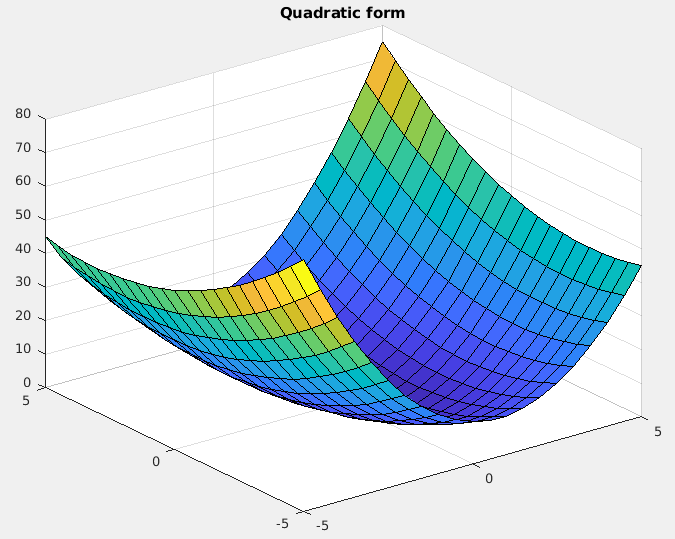
\includegraphics[width=0.7\columnwidth]{QuadraticForm.png}
	\caption{Plot of the surface produced by the quadratic form $f(u) = u^T A u$
		for arbitrarily-chosen symmetric matrix 
		$A = \bigl( \begin{smallmatrix} 1.9 & 0.3 \\ 0.3 & 0.5 \end{smallmatrix}\bigr)$.}
	\label{fig:QuadraticForm}
\end{figure}
More examples produced by random symmetric matrices are shown in \cref{fig:QuadraticForms_multiple}.
\begin{figure}[thb]
	\centering
	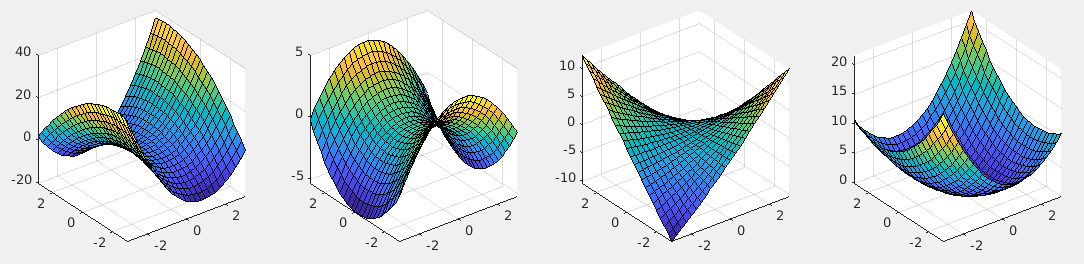
\includegraphics[width=1.0\columnwidth]{QuadraticForms_multiple.png}
	\caption{Four different quadratic forms created by four different random matrices.}
	\label{fig:QuadraticForms_multiple}
\end{figure}


\subsection{Eigenvalues and eigenvectors}
Now that we have a matrix visualization involving quadratic forms, what
can we learn from it?  
The shape of the surface carries a lot of information about the matrix $A$.
\cref{fig:QuadraticFormFixedSurfaces} shows the surfaces obtained from four
different matrices:
\begin{enumerate}
	\item Upward opening paraboloid.  $A = \bigl( \begin{smallmatrix} 1 & 0 \\ 0 & 1 \end{smallmatrix}\bigr)$.  Eigenvalues $\lambda_1 = \lambda_2 = 1$.
	\item Downward opening paraboloid.  $A = \bigl( \begin{smallmatrix} -1 & 0 \\ 0 & -1 \end{smallmatrix}\bigr)$.  Eigenvalues $\lambda_1 = \lambda_2 = -1$.
	\item Saddle (hyperbolic paraboloid). $A = \bigl( \begin{smallmatrix} 0 & 1 \\ 1 & 0 \end{smallmatrix}\bigr)$.  Eigenvalues $\lambda_1 = 1, \lambda_2 = -1$.
	\item Cylindrical paraboloid (degenerate form -- singular matrix). $A = \bigl( \begin{smallmatrix}  1 & 1 \\ 1 & 1 \end{smallmatrix}\bigr)$.  Eigenvalues $\lambda_1 = 2, \lambda_2 = 0$.
\end{enumerate}
\begin{figure}[thb]
	\centering
	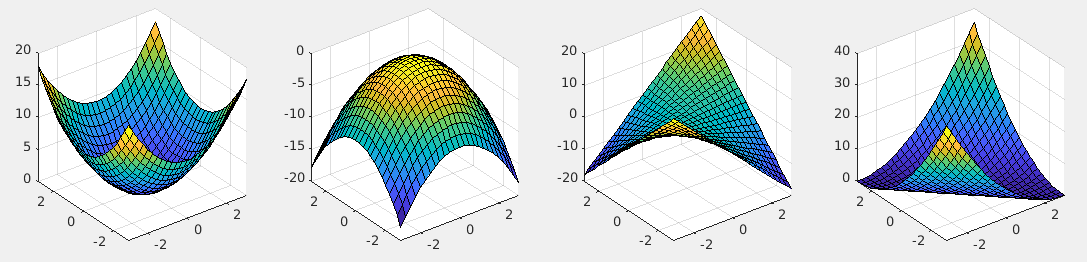
\includegraphics[width=1.0\columnwidth]{QuadraticFormFixedSurfaces.png}
	\caption{From left to right:  1. Upward opening paraboloid: the matrix is positive definite, 
		both eigenvalues are positive.  2. Downward opening paraboloid: the matrix is
		negative definite, both eigenvalues are negative.  3. Saddle:  The matrix is indeterminate,
		one eigenvalue is positive, one is negative.  4. Cylidrical paraboloid: The matrix is
		singular, one eigenvalue is positive, the other is zero.}
	\label{fig:QuadraticFormFixedSurfaces}
\end{figure}
The question is, is there a way to characterize each matrix which predicts something about
the quadratic form surfaces it creates?  The answer is yes, and the characterization involves
the eigenvalue decomposition (EVD) of the matrix,
\begin{equation}
\label{eq:evd}
A = Q \Lambda Q^T
\end{equation}
where $Q$ is an orthonormal matrix, and $\Lambda$ is a diagonal matrix whose diagonal elements
are the eigenvalues of matrix $A$.  I will assume you have some basic familiarity with
eigenvalues and eigenvectors; the subject is well treated in the standard linear algebra
textbooks.  One important thing to note is that by restricting ourselves to real, symmetric
matrices, the matrices $Q$ are automatically orthonormal and the eigenvalues are real.  These nice
properties are not guaranteed for random, non-symmetric matrices.  This is a big reason we have
restricted ourselves to real, symmetric matrices in this section.

Here are the points to notice about quadratic forms and the EVD:
\begin{itemize}
	\item The surface produced by $u^T A u$ is characterized by two curvatures in two orthogonal
	directions.  Positive curvature corresponds to an upward-facing parabola and negative curvature 
	corresponds to a downward-facing parabola.  In this case, "curvature" refers to the second
	derivative of the surface along a particular line passing through the origin.
	\item The signs of the two eigenvalues of $A$ correspond to the two curvature directions 
	of the surface.  A positive eigenvalue corresponds to an upward-facing parabola and a negative 
	eigenvalue corresponds to a downward-facing parabola.  If an eigenvalue is zero, it corresponds
	to one direction of the surface which faces neither up nor down -- this is the degenerate case shown
	in \cref{fig:QuadraticFormFixedSurfaces}
	\item The two directions of principle curvature are given by the eigenvectors of $A$. The
	term "principle curvature" means the minimum and maximum values of curvature along all 
	lines passing through the origin.  
	\item A positive definite matrix is one whose eigenvalues are all positive.  Such matrices
	show up frequently in real-world problems.  For a 2x2 matrix the corresponding surface is a paraboloid opening
	upward, such as is shown in \cref{fig:QuadraticFormFixedSurfaces}.   
	For 3x3 and higher dimensionality matrices the same holds true, except we can't
	visualize them since we can't visualize surfaces in 4 and higher dimensions.
	\item A negative definite matrix is one whose eigenvalues are all negative.  For a
	2x2 matrix the corresponding surface is a paraboloid opening downward, similar to
	the example shown in \cref{fig:QuadraticFormFixedSurfaces}. 
	\item A matrix whose eigenvalues have mixed sign is referred to as "indefinite".  The
	corresponding surface is a saddle, also shown in \cref{fig:QuadraticFormFixedSurfaces}.
\end{itemize}
In summary, the eigenvalues of $A$ predict what type of surface will be
obtained and the eigenvectors of $A$ predict the directions of maximum and minimum curvature.

%%%%%%%%%%%%%%%%%%%%%%%%%%%%%%%%%%%%%%%%%%%%%%%%%%%%%%%%%%%%%%%%%%%%%%%%%%%%%%
%XXXX  Need drawing showing vertical plates cutting paraboloid giving parabolas 
%XXXX  Need drawing showing how eigenvectors align along directions of principle curvature.


%%%%%%%%%%%%%%%%%%%%%%%%%%%%%%%%%%%%%%%%%%%%%%%%%%%%%%%%%%%%%%%%%%%%%%%%%%
% Need section on convergence of conjugate gradient

\subsection{Relation between ellipse and quadratic form visualizations}
Consider the case where matrix $A$ is positive definite.  The associated quadratic
form is an upward-opening paraboloid.  Now consider slicing the paraboloid with
planes parallel to the x-y plane as shown in \cref{fig:LevelsetsOfParabola}.  The
lines of intersection between the paraboloid and the slicing planes are called 
"levelsets" in optimization speak, or the "isolines" in computer graphics speak.  
Importantly for us, the lines are manifestly ellipses -- a fact that should
immediately remind us of the ellipse visualization presented in \cref{sec:unit_ball}.
\begin{figure}[thb]
	\centering
	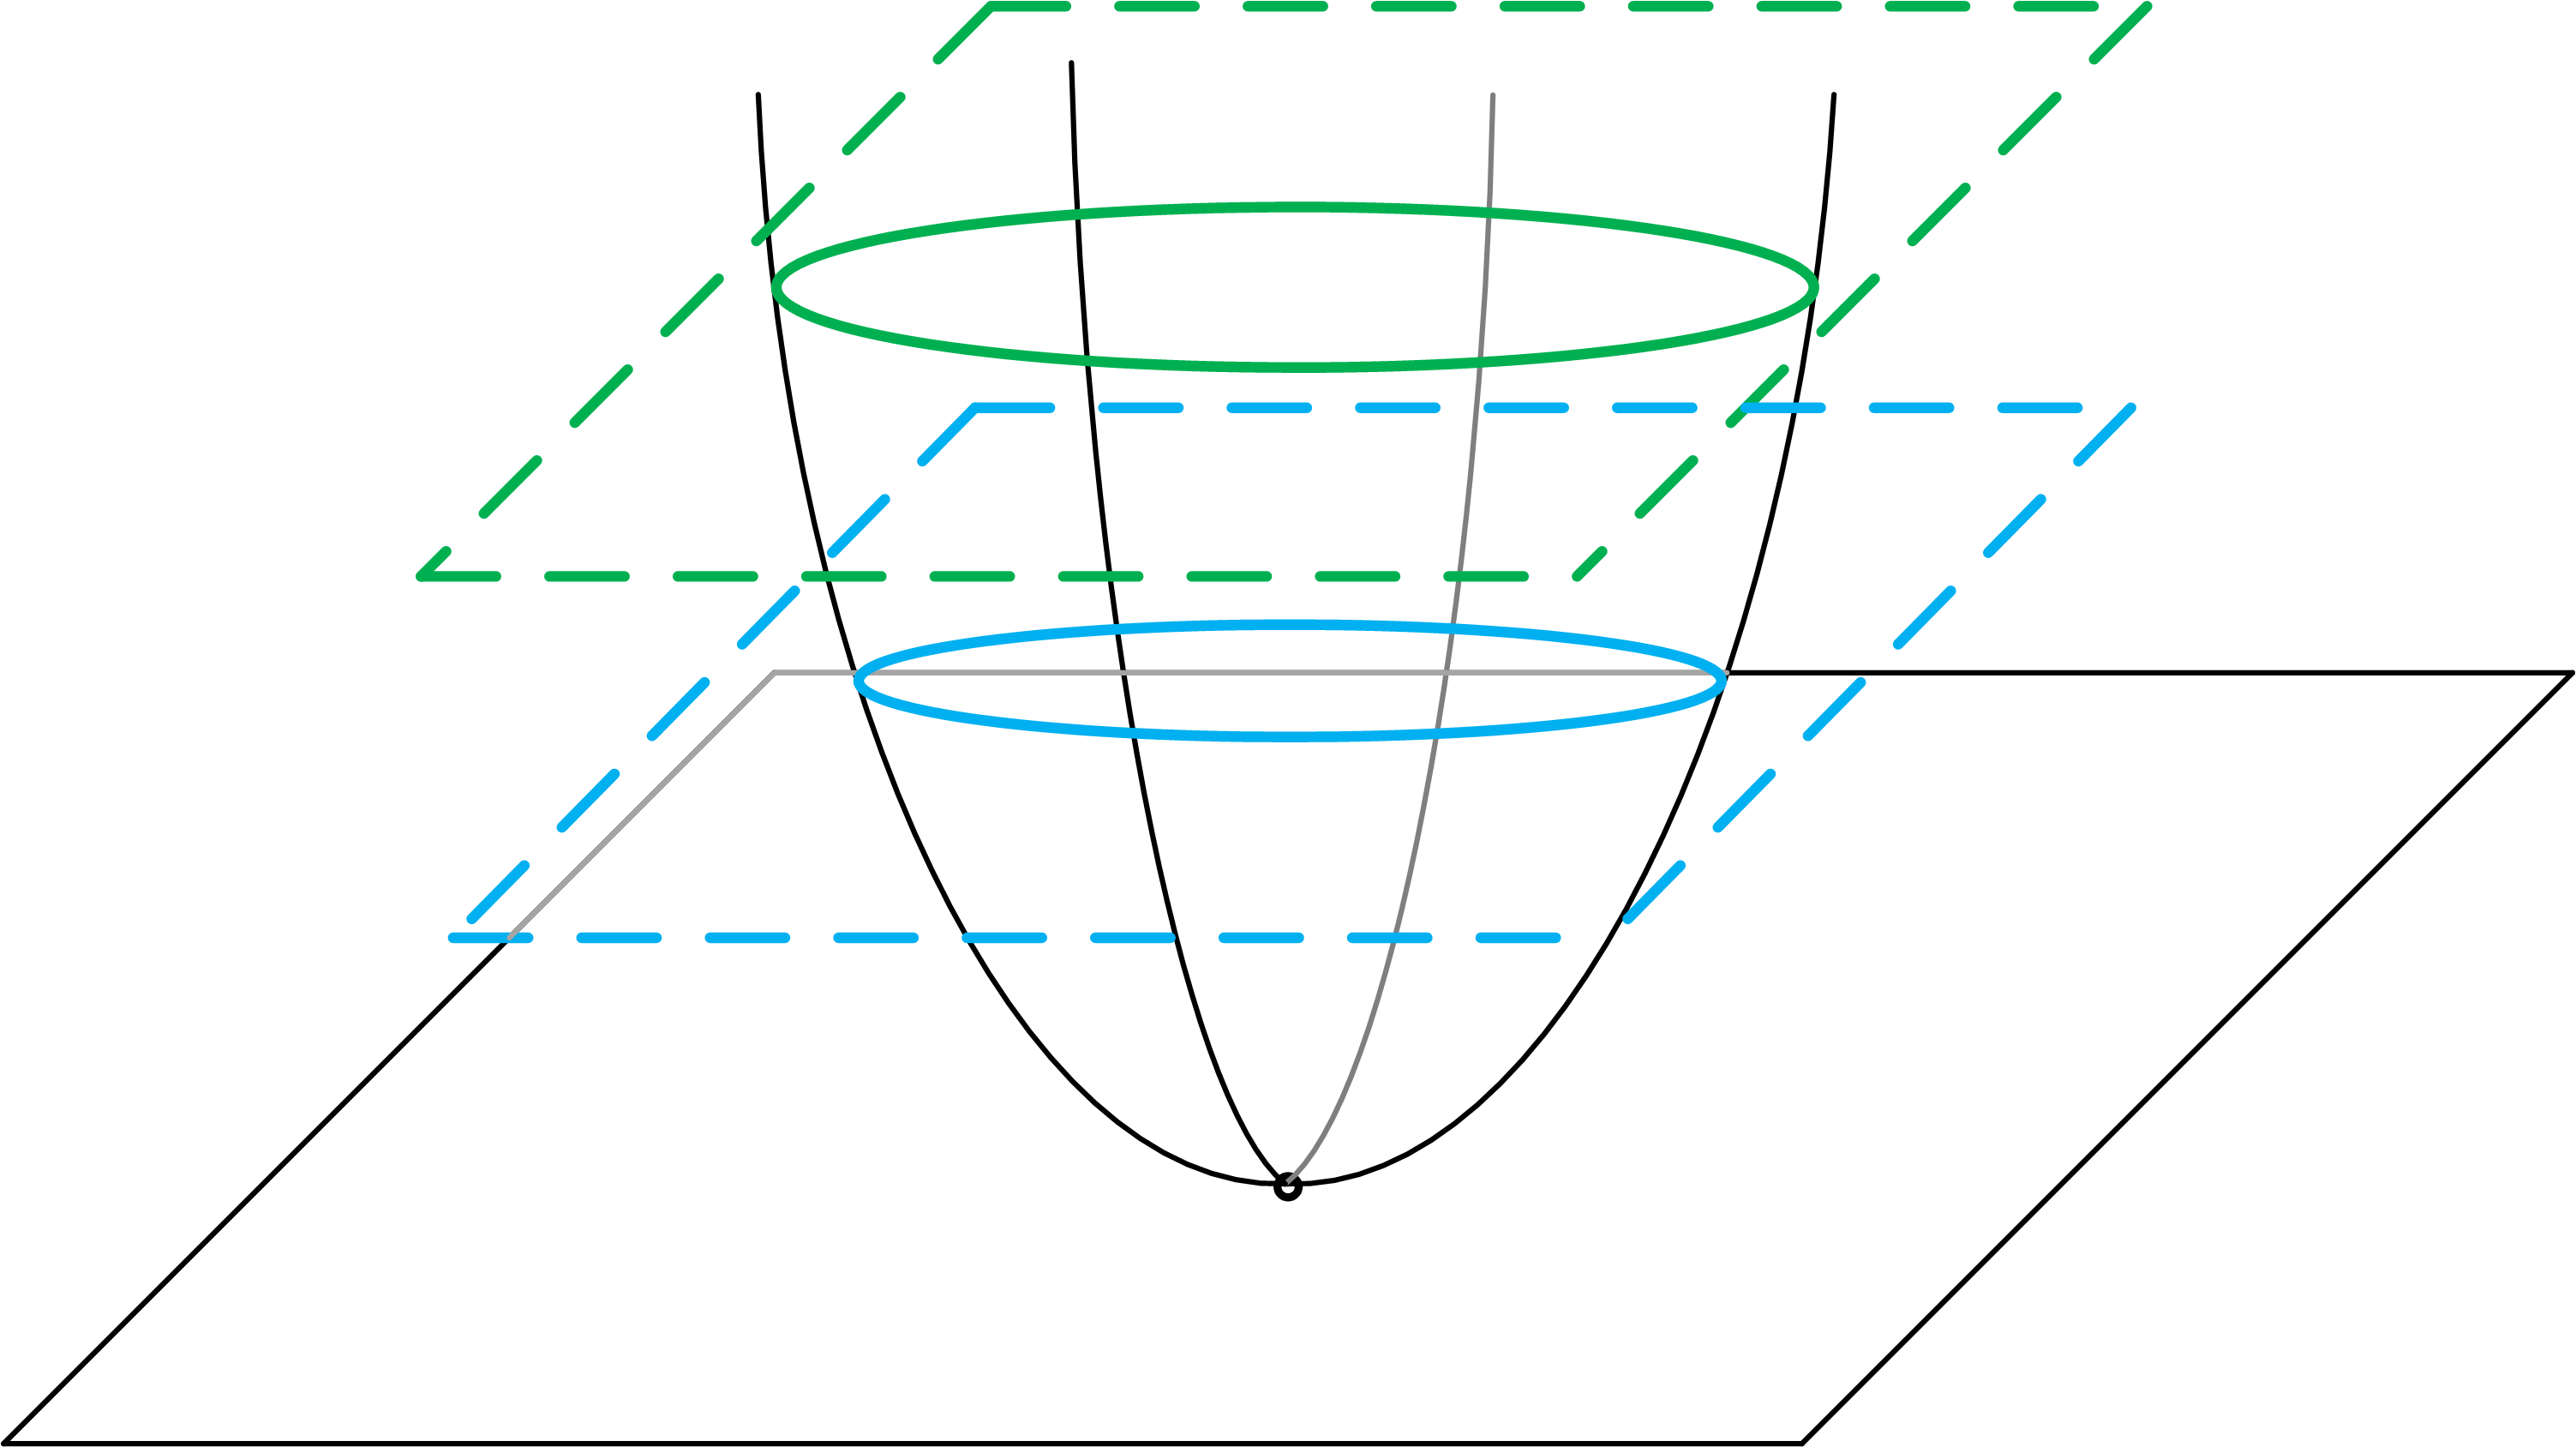
\includegraphics[width=0.7\columnwidth]{LevelsetsOfParabola.png}
	\caption{The levelsets (isolines) of the sliced paraboliod are
		ellipses, shown here as solid green and blue lines corresponding
		to different slicing planes.}
	\label{fig:LevelsetsOfParabola}
\end{figure}
The natural question is, is there a relationship between these ellipses and 
the ellipses generated by matrix-vector multiplication studied in \cref{sec:unit_ball}?
The answer is yes, the isoline ellipses depicted in \cref{fig:LevelsetsOfParabola} 
and the ellipses depicted in 
\cref{fig:CircleTransformedToEllipse} are indeed related.
However, the relationship is not as straightforward
as you might think.  The goal of this subsection is to derive the relationship.

First, recall that the isoline ellipses are described by the following equation:
\begin{equation}
u^T A u = c
\label{eq:quad_form}
\end{equation}
where the constant $c$ measures the height of the cutting plane off the "ground" 
(i.e. the $z = 0$ plane).  For what follows take $c=1$.
Next imagine that $A$ may be decomposed into a product
$A = B^T B$.  Since $A$ is positive definite we know this is the case --
the decomposition is essentially the Cholesky decomposition  \cite{Higham2020_Chol}.
Using this, \cref{eq:quad_form} becomes
\begin{equation}
1 = u^T B^T B u \\
= (u^T B^T) (B u) \\
= e^T e
\end{equation}
where $e = B u$ is a vector.  This equation says that the 2-norm of $e$ is one.  
Therefore, the set of all vectors $e$ are unit vectors, and their tips lie on the the unit circle.
This was the starting point of the ellipse visualization back in section \cref{sec:unit_ball}!  That
means the ellipses defined by \cref{eq:quad_form} are created by the matrix-vector
multiplication
$$
u = B^{-1} e
$$
where $e$ is the unit circle and $B$ is derived from $A$ via $A = B^T B$.

So the the isoline ellipses and the ellipses generated from the unit circle
under matrix-vector multiplication are indeed related.  But can we find a straightforward
forumula connecting them?  Consider the image of the unit circle under $A$,
$$
w = A e
$$
where $e$ is the unit circle and $w$ is its image as an ellipse.  Knowing that, and using
the definition of $B$ we have
$$
w = B^T B e \\
=  B^T B B u
$$
This says that $w$ is the image of $u$ under matrix-vector multiplication.  In particular,
the first product $B u$ returns a unit circle, and then $B^T B$ transforms it into
the ellipse $w$.  The relationship between $u$ and $w$ 
is depicted in \cref{fig:IsolineVsLinTransform}, which shows the two ellipses,
with each computed in two ways:
\begin{enumerate}
	\item The isoline defined by $1 = u^T A u$ and the ellipse
	derived from the unit circle $u = B^{-1} e$.
	\item The ellipse generated from the transform of the unit circle
	$y = A e$ and the transform of the ellipse in item 1, 
	$w = B^{T} B B u$.
\end{enumerate}
\begin{figure}[bht]
	\centering
	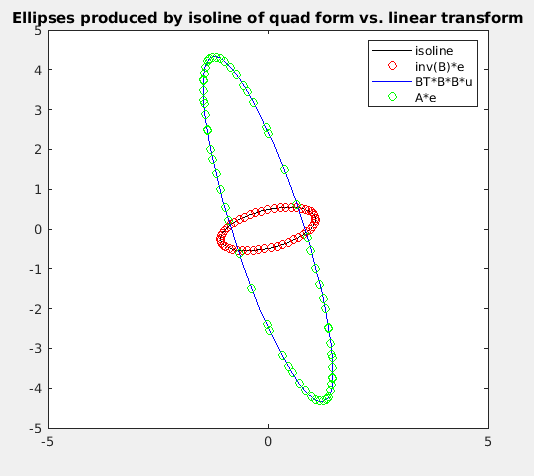
\includegraphics[width=0.7\columnwidth]{IsolineVsLinTransform.png}
	\caption{Four ellipses associated with matrix $A$:  two generated
		by the quadratic form, and two generated by the
		linear transform visualization.}
	\label{fig:IsolineVsLinTransform}
\end{figure}

\subsection{Condition number and the quadratic form visualization}
Recall using the ellipse visualization in \cref{conditionnumber} as 
a proxy of the condition number.  Can we also use the quadratic form
visualization as a way to understand the condition number of $A$?  As usual,
when I ask a rhetorical question in this article the answer is "yes".

The keys to this visualization are the eigenvalues of $A$.  It can be shown that
the eigenvalues of a symmetric, positive definite matrix are equal to its singular
values, $\lambda_i = \sigma_i$.  Therefore, the condition number of $A$ is
$$
\kappa = \frac{\sigma_{max}}{\sigma_{min}} = \frac{\lambda_{max}}{\lambda_{min}}
$$
Recall that the curvature of the paraboloid generated by $f(u) = u^T A u$ in any of
the principal directions is proportional to the corresponding eigenvalue $\lambda_i$.
The larger the $\lambda_i$, the larger is the curvature, so the tighter is the 
parabola.  The smaller the $\lambda_i$, the smaller is the curvature, and so the more open is the 
parabola.  
\begin{figure}[bht]
	\centering
	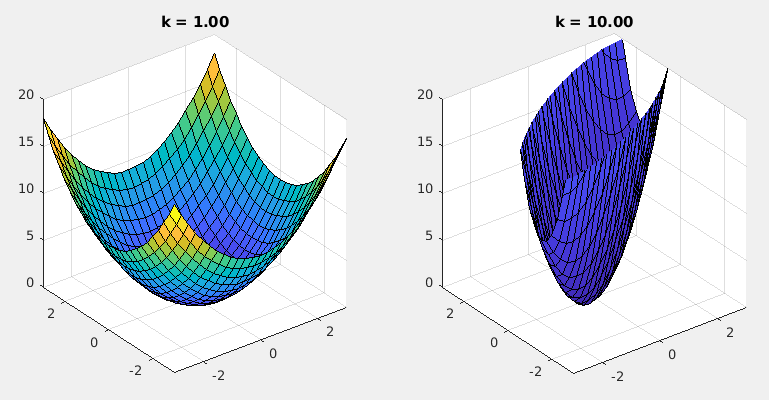
\includegraphics[width=0.8\columnwidth]{QuadFormCondNo.png}
	\caption{On the left is a paraboloid generated by a matrix with condition
		number $\kappa = 1$.   On the right is a paraboloid generated by a matrix with condition
		number $\kappa = 10$.}
	\label{fig:QuadFormCondNo}
\end{figure}
This effect is shown in \cref{fig:QuadFormCondNo} which shows the paraboloids generated
by two different $A$ matrices, one with condition number 1 and the other with condition
number 10.  The paraboloid with condition number 10 is quite clearly squeezed in one direction
since its principal curvature in that direction is high.  The squeezed parabola causes
some iterative algorithms like gradient descent to converge slowly, but that is a topic for
a different article.


\section{Summary and review}
This paper has presented a guided tour of different ways to think about
a matrix in geometric terms.  Here is a summary of different matrix visualizations
provided by this article:
\begin{itemize}
\item Visualize the action of a matrix $A$ transforming the unit square 
into a parallelogram as shown in \cref{fig:MatrixActionOnUnitSquare}.  
The parallelogram's area is given
by the determinant of the input matrix $A$.  

\item Visualize the action of a matrix $A$ transforming the unit circle centered at the
origin.  The result is an ellipse as shown in \cref{fig:CircleTransformedToEllipse}.  
The lengths of the axes of the ellipse 
are given by the singular values $\Sigma$ generated by the SVD of $A$, $A = U \Sigma V^T$.

\item Imagine the action of the decomposed matrix $A = U \Sigma V^T$ as three separate
actions: 1.  Rotation by $V^T$, 2.  stretching by $\Sigma$, 3.   a final rotation by $U$.
This is shown in \cref{fig:ActionOfSVDOnCircle}

\item Specializing to the case of real, symmetric $A$, visualize the
surface created by the quadratic form $f(u) = u^T A u$.  Examples are shown in 
\cref{fig:QuadraticFormFixedSurfaces}.  The exact shape taken
by the surface (paraboloid, saddle, etc.) depends upon the eigenvalues of $A$.

\item A final visualization applies to a positive definite matrix:  the
 cutting planes intersecting the quadratic form $f(u) = u^T A u$ form an ellipse,
\cref{fig:LevelsetsOfParabola}.  
The ellipse is not the same size nor shape as that found by 
matrix-vector multiplication, but the two ellipses are related via Cholesky decomposition of matrix $A$.
\end{itemize}
My experience is that these visualizations give me insights into the behavior
of numerical problems.  I hope you find them useful too as you continue
your mathematical studies.

\appendix
\section{Matlab codes}
\hbadness=99999 

\subsection{Action of a random matrix on a unit square}
\label{mat:ActionUnitSquare}
\begin{verbatim}
function transform_square()
  % This function takes a set of points forming a
  % unit square x and plots it.  Then it generates 
  % a random 2x2 matrix, A, and forms the product
  % y = A*x.  It then plots the product 
  % on the same plot.

  % Create unit square from 4 sides
  N = 625;  % Number of points per side
  s = linspace(0,1,N);
  z = zeros(size(s));
  o = ones(size(s));
  
  % Create points. Each point is a 2-element column 
  % vector, [x;y]; the points are concatenated into 
  % a short, fat 2xN matrix  which holds all the 
  % points in the square.
  s1 = [s;z]; % bottom
  s2 = [o;s]; % right side
  s3 = [s;o]; % top
  s4 = [z;s]; % left side
  x = [s1,s2,s3,s4];   % square

  % Plot square
  plot(x(1,:), x(2,:), 'ro', 'MarkerFaceColor', ...
    'red', 'MarkerSize', 0.5)
  hold on
  axis([-3, 3, -3, 3]);

  % Now create random 2x2 matrix A.  The elements 
  % have mean 0 and variance 1.
  A = randn(2,2);

  % Now compute matrix-vector product and plot it.
  y = A*x;
  oldplot = plot(y(1,:), y(2,:), 'bo', 'MarkerFaceColor', ...
    'blue', 'MarkerSize', 0.5); 

  % Report det(A)
  fprintf('det(A) = %f\n', det(A))
end
\end{verbatim}

\subsection{Action of a random matrix on a unit circle}
\label{Mat:ActionUnitBall}
\begin{verbatim}
function A = ellipses()
  % This fcn generates a random 2x2 matrix A, and 
  % then applies it to the unit circle.  It then 
  % plots the result.  The goal is to visualize a 
  % matrix via its transformation of a unit
  % circle (or ball in ND).

  % Create unit circle u (parameterized by theta)
  theta = linspace(0, 2*pi, 50);
  u = [cos(theta); sin(theta)];  % Column vector

  % Now create random 2x2 matrix, and apply it to u.
  A = randn(2);
  v = A*u;

  plot(u(1, :), u(2, :), 'r')  % Reference circle is red
  hold on
  plot(v(1, :), v(2, :), 'b')  % Transformed circle is blue
  axis([-3, 3, -3, 3], 'square');
end
\end{verbatim}

\subsection{Condition number theorem}
\label{Mat:CondThm}

\begin{verbatim}
function test_cond_thm(k)
  % Input: k = condition number of matrix to make

  for i=1:10
    N = 5;
    A = randn_cond(N,N,k);
    x = randn(N,1);
    b = A*x;

    db = randn(N,1)/eps(1);
    bt = b + db;
    xt = A\bt;

    relfwderr = norm(xt-x)/norm(x);
    relbkwderr = norm(bt-b)/norm(b);
    kcomputed = relfwderr/relbkwderr;

    fprintf('k input = %f, k computed = %f \n', k, kcomputed)
  end

end
\end{verbatim}


%\section{References}
%\bibliographystyle{siamplain}
%\bibliography{references}

\begin{thebibliography}{9}
	
\bibitem{Weisstein_MatrixNorm} Eric W. Weisstein, "Matrix Norm." From MathWorld--A Wolfram Web Resource.  \url{https://mathworld.wolfram.com/MatrixNorm.html}

\bibitem{higham2020_svd} Nick Higham, "What Is the Singular Value Decomposition?", \url{https://nhigham.com/2020/10/13/what-is-the-singular-value-decomposition/}
	
\bibitem{higham2020_OrthoMatrix} Nick Higham, "What is an orthogonal matrix?", \url{https://nhigham.com/2020/04/07/what-is-an-orthogonal-matrix/}

\bibitem{Moler2014_FloatingPoint} Cleve Moler, "Floating Point Numbers", \url{https://blogs.mathworks.com/cleve/2014/07/07/floating-point-numbers/}

\bibitem{moler2017} Cleve Moler, "What is the condition number of a matrix?", \url{https://blogs.mathworks.com/cleve/2017/07/17/what-is-the-condition-number-of-a-matrix/}

\bibitem{Higham2020_BkwdErr} Nick Higham, "What Is Backward Error?", \url{https://nhigham.com/2020/03/25/what-is-backward-error/}

\bibitem{Trefethen97} For a full discussion, see L. Trefethen, and D. Bau,
"Numerical Linear Algebra", 
SIAM, Philadelphia, (1997)

\bibitem{Higham2020_Chol} Nick Higham,  "What Is a Cholesky Factorization?",  \url{https://nhigham.com/2020/08/11/what-is-a-cholesky-factorization/}

\end{thebibliography}

% Cond no.
% 
% https://github.com/higham/what-is/blob/master/cond.pdf

% SVD
% https://www.mathworks.com/company/newsletters/articles/professor-svd.html
 % https://github.com/higham/what-is/blob/master/svd.pdf


\end{document}
